\documentclass[letter, 12pt, epsf]{article}
\usepackage[outdir=./]{epstopdf}
\usepackage{setspace}
\usepackage{graphics}
\usepackage{graphicx}
\usepackage{amssymb}
\usepackage{amsmath}
\usepackage{theorem}
\usepackage{anysize}
\usepackage[T1]{fontenc}
\usepackage[sc]{mathpazo}
\usepackage{calligra}
\linespread{1.05}   %
\usepackage{epsfig}
\usepackage{subfigure}
\usepackage{color}
\usepackage{xcolor}
\usepackage{verbatim}
\usepackage{multirow}
%\usepackage{float}
\usepackage{caption}
%\usepackage{subcaption}
%\usepackage{subfig}
%\usepackage{subfloat}
\usepackage[section]{placeins}
\usepackage{booktabs}
\usepackage{soul}
\usepackage{floatrow}
\floatsetup[table]{capposition=top}
\usepackage{booktabs}
\usepackage{threeparttable}
\usepackage{array}
\usepackage{longtable}
\usepackage{natbib}
\DeclareGraphicsExtensions{.eps}
\DeclareUnicodeCharacter{FB01}{fi}
\setcounter{topnumber}{2}
\setcounter{bottomnumber}{2}
\setcounter{totalnumber}{4}
\renewcommand{\topfraction}{0.85}
\renewcommand{\bottomfraction}{0.85}
\renewcommand{\textfraction}{0.15}
\renewcommand{\floatpagefraction}{0.7}
\newcommand{\sym}[1]{{#1}} % for symbols in Table


%\usepackage{booktabs}
\usepackage{threeparttable}
\usepackage{array}
\newtheorem{prop}{Proposition}
\newtheorem{lem}{Lemma}
%\newtheorem{pro}{Proof}\mathds{}
\newtheorem{thm}{Theorem}
\newtheorem{defn}{Definition}
\newtheorem{corr}{Corollary}
\theorembodyfont{\rmfamily} \linespread{1.4}
\newtheorem{con}{Conjecture}
\newtheorem{rem}{Remark}
\newtheorem{exa}{Example}

\usepackage[a4paper,bindingoffset=0.2in,%
            left=1in,right=1in,top=1in,bottom=1in,%
            footskip=.25in]{geometry}

\usepackage{hyperref}
\hypersetup{%
    colorlinks=true, linktocpage=true, pdfstartpage=3, pdfstartview=FitV,%
    breaklinks=true, pdfpagemode=UseNone, pageanchor=true, pdfpagemode=UseOutlines,%
    plainpages=false, bookmarksnumbered, bookmarksopen=true, bookmarksopenlevel=1,%
    hypertexnames=true, pdfhighlight=/O,hyperfootnotes=true,%nesting=true,%frenchlinks,%
    urlcolor=blue, linkcolor=blue, citecolor=blue, %pagecolor=RoyalBlue,%
    pdftitle={Article},%the title
    pdfauthor={Enchuan Shao, Pedro Silos},%your name
    pdfsubject={},%
    pdfkeywords={},%
    pdfcreator={XeLaTeX},%
    pdfproducer={A happy XeLaTeX user}%
}
\begin{document}

%{
\def\sym#1{\ifmmode^{#1}\else\(^{#1}\)\fi}
\begin{tabular}{l*{6}{c}}
\hline\hline
                    &\multicolumn{1}{c}{(1)}&\multicolumn{1}{c}{(2)}&\multicolumn{1}{c}{(3)}&\multicolumn{1}{c}{(4)}&\multicolumn{1}{c}{(5)}&\multicolumn{1}{c}{(6)}\\
                    &\multicolumn{1}{c}{Weekday}&\multicolumn{1}{c}{Weekend}&\multicolumn{1}{c}{Weekday}&\multicolumn{1}{c}{est4}&\multicolumn{1}{c}{est5}&\multicolumn{1}{c}{est6}\\
\hline
Female Gap in Work Hours&      -0.898\sym{***}&      -0.749\sym{***}&      -0.901\sym{***}&      -0.911\sym{***}&      -0.703\sym{***}&      -0.490\sym{***}\\
                    &    (0.0694)         &    (0.0674)         &    (0.0692)         &    (0.0702)         &    (0.0698)         &    (0.0768)         \\
\hline
Observations        &       12113         &       12344         &       12113         &       12113         &       12113         &        8393         \\
\hline\hline
\end{tabular}
}
                    &\multicolumn{1}{c}{Weekday}&\multicolumn{1}{c}{Weekend}\\
\hline
Male                &       7.904&       2.163\\
                    &            &            \\
[1em]
Female              &       7.006&       1.414\\
                    &            &            \\
[1em]
Total               &       7.611&       1.906\\
                    &            &            \\
\hline
Observations        &       12113&       12344\\

%{
\def\sym#1{\ifmmode^{#1}\else\(^{#1}\)\fi}
\begin{tabular}{l*{6}{c}}
\hline\hline
                    &\multicolumn{1}{c}{(1)}&\multicolumn{1}{c}{(2)}&\multicolumn{1}{c}{(3)}&\multicolumn{1}{c}{(4)}&\multicolumn{1}{c}{(5)}&\multicolumn{1}{c}{(6)}\\
                    &\multicolumn{1}{c}{Weekday}&\multicolumn{1}{c}{Weekend}&\multicolumn{1}{c}{Weekday}&\multicolumn{1}{c}{est4}&\multicolumn{1}{c}{est5}&\multicolumn{1}{c}{est6}\\
\hline
Female Gap in Household Hours&       0.436\sym{***}&       0.264\sym{***}&       0.436\sym{***}&       0.349\sym{***}&       0.319\sym{***}&       0.266\sym{***}\\
                    &    (0.0276)         &    (0.0332)         &    (0.0276)         &    (0.0270)         &    (0.0272)         &    (0.0327)         \\
\hline
Observations        &       12113         &       12344         &       12113         &       12113         &       12113         &        8393         \\
\hline\hline
\end{tabular}
}
                    &\multicolumn{1}{c}{Weekday}&\multicolumn{1}{c}{Weekend}\\
\hline
Male                &       0.821&       1.002\\
                    &            &            \\
[1em]
Female              &       1.257&       1.267\\
                    &            &            \\
[1em]
Total               &       0.963&       1.093\\
                    &            &            \\
\hline
Observations        &       12113&       12344\\

\begin{table}[!htbp]
\centering{
\caption{Work among Full-time Workers, Married with Children}\label{table1}
\scalebox{0.8}{
\small \begin{tabular}{l*{7}{c}}
\hline
                    &\multicolumn{1}{c}{Weekday}&\multicolumn{1}{c}{Weekend}&\multicolumn{1}{c}{Weekday}&\multicolumn{1}{c}{est4}&\multicolumn{1}{c}{est5}&\multicolumn{1}{c}{est6}\\
\hline
Female Gap in Work Hours&      -0.898\sym{***}&      -0.749\sym{***}&      -0.901\sym{***}&      -0.911\sym{***}&      -0.703\sym{***}&      -0.490\sym{***}\\
                    &    (0.0694)         &    (0.0674)         &    (0.0692)         &    (0.0702)         &    (0.0698)         &    (0.0768)         \\
\hline
Observations        &       12113         &       12344         &       12113         &       12113         &       12113         &        8393         \\
\hline\hline
                    &\multicolumn{1}{c}{Weekday}&\multicolumn{1}{c}{Weekend}\\
\hline
Male                &       7.904&       2.163\\
                    &            &            \\
[1em]
Female              &       7.006&       1.414\\
                    &            &            \\
[1em]
Total               &       7.611&       1.906\\
                    &            &            \\
\hline
Observations        &       12113&       12344\\
\multicolumn{8} {p{7.2in}} { {\footnotesize{
Notes:
Data are from the 2003-2014 American Time Use Surveys (ATUS). The table is based on 18-65 year old ATUS respondents who report working full-time in the activity summary file.  We keep those who are married with spouse present and have at least one own child in the household. The dependent variable is total hours spent on ``work and work-related activities'' on the diary day. Each column reports the coefficient on the ``female'' dummy. Column (5) controls for usual weekly hours worked reported in the activity summary file. Column (6) only includes workers who reported usual weekly hours of less than 50. Individual observations are weighted by ATUS weights for multi-year data files.
}}}
\end{tabular}
}}
\end{table}

\begin{figure}[htb]
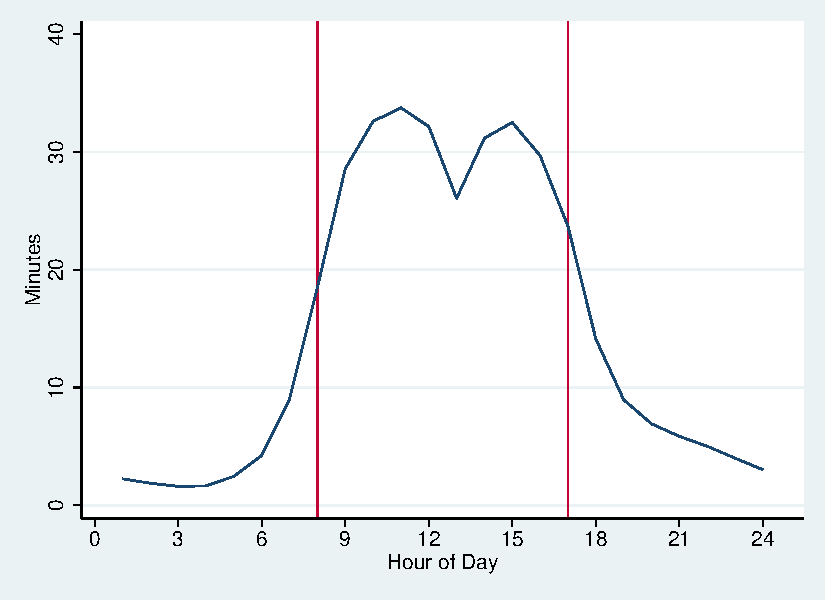
\includegraphics{./fig1.pdf}
\caption{}
\end{figure}

\begin{table}[!htbp]
\centering{
\caption{Work among Full-time Workers, Married with Children}\label{table1}
\scalebox{0.8}{
\small \begin{tabular}{l*{7}{c}}
\hline
                    &\multicolumn{1}{c}{Weekday}&\multicolumn{1}{c}{Weekend}&\multicolumn{1}{c}{Weekday}&\multicolumn{1}{c}{est4}&\multicolumn{1}{c}{est5}&\multicolumn{1}{c}{est6}\\
\hline
Female Gap in Household Hours&       0.436\sym{***}&       0.264\sym{***}&       0.436\sym{***}&       0.349\sym{***}&       0.319\sym{***}&       0.266\sym{***}\\
                    &    (0.0276)         &    (0.0332)         &    (0.0276)         &    (0.0270)         &    (0.0272)         &    (0.0327)         \\
\hline
Observations        &       12113         &       12344         &       12113         &       12113         &       12113         &        8393         \\
\hline\hline
                    &\multicolumn{1}{c}{Weekday}&\multicolumn{1}{c}{Weekend}\\
\hline
Male                &       0.821&       1.002\\
                    &            &            \\
[1em]
Female              &       1.257&       1.267\\
                    &            &            \\
[1em]
Total               &       0.963&       1.093\\
                    &            &            \\
\hline
Observations        &       12113&       12344\\
\multicolumn{8} {p{7.2in}} { {\footnotesize{
Notes:
Data are from the 2003-2014 American Time Use Surveys (ATUS). The table is based on 18-65 year old ATUS respondents who report working full-time in the activity summary file.  We keep those who are married with spouse present and have at least one own child in the household. The dependent variable is total hours spent on ``work and work-related activities'' on the diary day. Each column reports the coefficient on the ``female'' dummy. Column (5) controls for usual weekly hours worked reported in the activity summary file. Column (6) only includes workers who reported usual weekly hours of less than 50. Individual observations are weighted by ATUS weights for multi-year data files.
}}}
\end{tabular}
}}
\end{table}

\begin{figure}[htb]
    \begin{center}
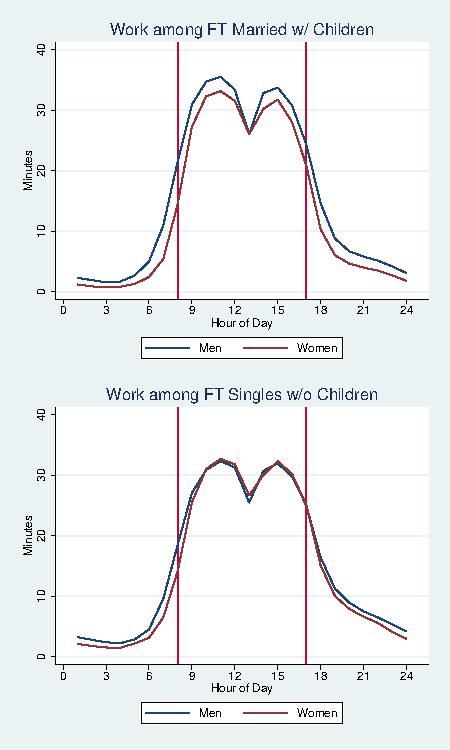
\includegraphics{./fig2.pdf}
\caption{}

\end{center}
\end{figure}
\begin{figure}[htb]
    \begin{center}
    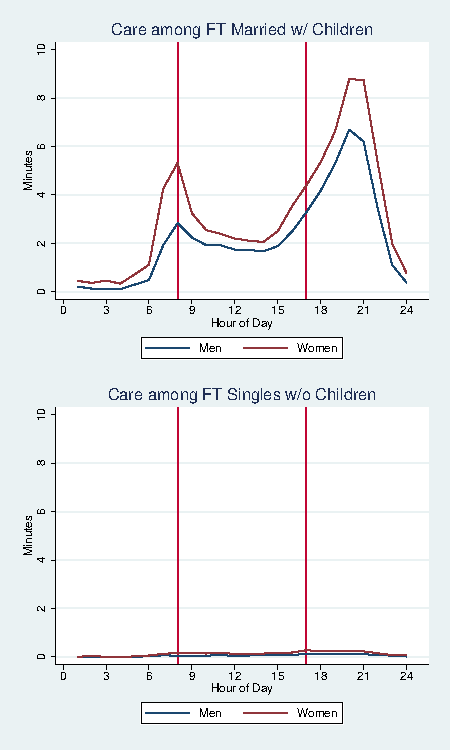
\includegraphics{./fig3.pdf}
\caption{}

\end{center}
\end{figure}
\begin{figure}[htb]
    \begin{center}
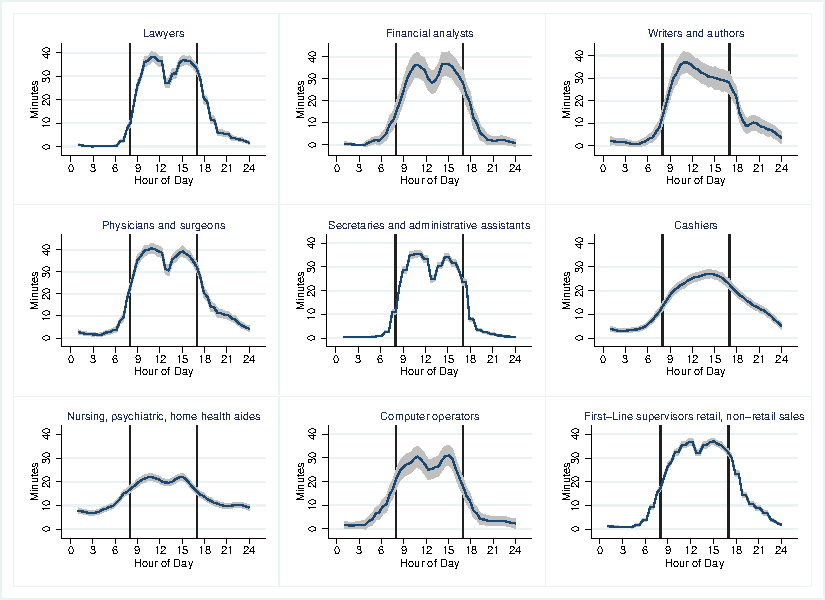
\includegraphics{./fig4.pdf}
\caption{}

\end{center}
\end{figure}







\def\sep{0.5em}
\defns{\footnotesize}
\begin{table}[htbp]\centering
\footnotesize
\caption{Household Care Activities of Parents by Marital and Work Status (Hours)}\label{table3}
\scalebox{0.8}{
\begin{tabular}{l  c c c c}
            &\multicolumn{1}{c}{(1)}&\multicolumn{1}{c}{(2)}&\multicolumn{1}{c}{(3)}&\multicolumn{1}{c}{(4)}\\
            &\multicolumn{1}{c}{Married\_NW}&\multicolumn{1}{c}{Married\_FT}&\multicolumn{1}{c}{Single\_FT}&\multicolumn{1}{c}{Male\_Married\_FT}\\
            &        b/se&        b/se&        b/se&        b/se\\
\hline
Routine     &         1.4&         1.0&         0.8&         0.4\\
            &      (0.03)&      (0.03)&      (0.04)&      (0.02)\\
Enrichment  &         0.6&         0.4&         0.3&         0.3\\
            &      (0.02)&      (0.02)&      (0.02)&      (0.01)\\
Other       &         0.4&         0.4&         0.4&         0.1\\
            &      (0.01)&      (0.01)&      (0.02)&      (0.01)\\
            &\multicolumn{1}{c}{(1)}&\multicolumn{1}{c}{(2)}&\multicolumn{1}{c}{(3)}&\multicolumn{1}{c}{(4)}\\
            &\multicolumn{1}{c}{Married\_NW}&\multicolumn{1}{c}{Married\_FT}&\multicolumn{1}{c}{Single\_FT}&\multicolumn{1}{c}{Male\_Married\_FT}\\
            &        b/se&        b/se&        b/se&        b/se\\
\hline
Routine     &         0.4&         0.2&         0.2&         0.1\\
            &      (0.01)&      (0.01)&      (0.01)&      (0.01)\\
Enrichment  &         0.6&         0.4&         0.3&         0.3\\
            &      (0.02)&      (0.01)&      (0.02)&      (0.01)\\
Other       &         0.4&         0.2&         0.3&         0.1\\
            &      (0.01)&      (0.01)&      (0.01)&      (0.01)\\
            &\multicolumn{1}{c}{(1)}&\multicolumn{1}{c}{(2)}&\multicolumn{1}{c}{(3)}&\multicolumn{1}{c}{(4)}\\
            &\multicolumn{1}{c}{Married\_NW}&\multicolumn{1}{c}{Married\_FT}&\multicolumn{1}{c}{Single\_FT}&\multicolumn{1}{c}{Male\_Married\_FT}\\
            &        b/se&        b/se&        b/se&        b/se\\
\hline
Routine     &         1.0&         0.9&         0.7&         0.4\\
            &      (0.02)&      (0.02)&      (0.03)&      (0.02)\\
Enrichment  &         0.4&         0.4&         0.3&         0.3\\
            &      (0.02)&      (0.02)&      (0.02)&      (0.01)\\
Other       &         0.1&         0.1&         0.1&         0.1\\
            &      (0.01)&      (0.01)&      (0.01)&      (0.00)\\
            &\multicolumn{1}{c}{(1)}&\multicolumn{1}{c}{(2)}&\multicolumn{1}{c}{(3)}&\multicolumn{1}{c}{(4)}\\
            &\multicolumn{1}{c}{Married\_NW}&\multicolumn{1}{c}{Married\_FT}&\multicolumn{1}{c}{Single\_FT}&\multicolumn{1}{c}{Male\_Married\_FT}\\
            &        b/se&        b/se&        b/se&        b/se\\
\hline
Routine     &         0.2&         0.1&         0.1&         0.1\\
            &      (0.01)&      (0.01)&      (0.01)&      (0.00)\\
Enrichment  &         0.5&         0.4&         0.4&         0.3\\
            &      (0.02)&      (0.01)&      (0.02)&      (0.01)\\
Other       &         0.1&         0.1&         0.1&         0.1\\
            &      (0.01)&      (0.01)&      (0.01)&      (0.00)\\
\hline \multicolumn{5} {p{6.2in}}
            {{\footnotesize{Note:
            Data are from the 2003-2014 American Time Use Surveys
(ATUS). The table shows the average hours allocated to household care
activities by parents. See main text for the definitions of the main
activities. See Appendix for
detailed activities that are included in each category. Married NW
refers to married women with spouse present who are not working,
Married FT refers to men and women who are married with spouse present
and working full-time, Single FT refers to single women who are
working full-time.   }}}
\end{tabular}
}
\end{table}

\def\sep{0.5em}
\begin{table}[!htbp]
\centering {
\caption{Correlations between Importance of Occupational Characteristics and Ratio8to5}\label{table4}
 \scalebox{0.8}{

\small\begin{tabular}{clc}\\
\hline
& &\\
$\#$Cat.&Name: O*NET Characteristic& Corr. Coeff.\\[\sep]
\hline
1&Assisting and caring for others & -0.1908\sym{*}\\[\sep]
2&Coaching and developing others &0.0471\\[\sep]
3&Developing\_and\_Building\_Teams &0.0525\\[\sep]
4&Establishing\_and\_Maintaining\_Interpersonal\_Relationships &0.2948\sym{*}\\[\sep]
5&Face-to-Face\_Discussions &0.2336\sym{*}\\[\sep]
7&Social orientation &0.0471\\[\sep]
8&Training\_and\_Teaching\_Others &-0.0719\\[\sep]
10&Guiding\_Directing\_and\_Motivating\_Subordinates &0.0501\\[\sep]

\hline
& &\\
&Concentration Index                                 &0.7430\sym{*}\\[\sep]
&Male Overwork                                       &0.1290\sym{*}\\
& &\\
\hline
& &\\
$\#$Cat.&Name: O*NET Skill Measures& Corr. Coeff.\\[\sep]
\hline
1&Social Skills &0.2129\sym{*}\\[\sep]
2&Abstract Skills &0.3632\sym{*}\\[\sep]
3&Manual Skills &-0.4362\sym{*}\\[\sep]
4&Routine Skills &-0.3737\sym{*}\\[\sep]
\hline
\multicolumn{3} {p{6in}} { {\footnotesize{
Notes:
The
table shows correlations between our standardized Ratio8to5 and O*NET
occupational characteristics for 434 detailed Census 2002 occupations.
Ratio8to5 is the ratio of total hours worked by all full-time workers
during the hours 8 a.m. to 5 p.m. relative to total hours worked in
each occupation category in the ATUS time diary data. See Appendix for
the detailed definitions of the O*NET
characteristics, as well as for details on the variables used and for
matching across O*NET Standard Occupation Codes (SOC) and 2002 Census
occupation codes. (*) denotes
significance at the 5\% level.  }}}
\end{tabular}
}}
\end{table}

\begin{table}[ht]
\centering
\caption{A Simple Case with Gender Differences} \label{table7}
\scalebox{0.85}{
\begin{tabular}{lccccccc}  \hline
\\
\footnotesize{
Occupation}          & \footnotesize{$\%$ Workers}&\footnotesize{Bunching Ratio}   &\footnotesize{Earnings}   &\footnotesize{$l_1+l_2$}&  \footnotesize{$l$}   & \footnotesize{$\%$ Females}& \footnotesize{E. Gap}\\ \\
(1)                 & (2)         &       (3)       &  (4)   &(5)      &  (6)   & (7)&(8)\\
\hline\\\\
       \multicolumn{8}{l}{\footnotesize Panel A: No Gender Differences}\\
\hline\\
1              & 0.48      &  0.59     &  0.42      &   0.82 &  0.80  &             & \\
2              & 0.52       &  0.51      &  0.38       &   0.80 &  0.80  &           &\\
 \hline \\
                      \multicolumn{8}{l}{\footnotesize Panel B: Gender-Specific
				  $
u$}\\
\hline\\
1              & 0.44       &  0.55      &  0.46       &   0.91 &  0.90  & 0           &\\
2              & 0.56       &  0.52      &  0.36       &   0.73 &  0.73 &89         & 1.005 \\
\\
Gender Earnings Gap  &\multicolumn{7}{l}{1.031}\\
\hline \\\\
                      \multicolumn{8}{l}{\footnotesize Panel C: Gender-Specific
					  $\nu$ and Tastes}\\
\hline\\
1              & 0.50       &  0.60      &  0.40       &   0.81  &  0.80   & 50    & 1.047       \\
2              & 0.50       &  0.51      &  0.40       &   0.81  &  0.80   & 50    &1.005      \\
\\
Gender Earnings Gap  &\multicolumn{7}{l}{1.026}
\\
\hline
\\
\multicolumn{8} {p{6.8in}} { {\footnotesize{
}}}
\end{tabular}
}
\end{table}

\input{./table6_fixed.tex}
\input{./table7_fixed.tex}
\def\sep{0.5em}
\def\fns{\footnotesize}
\begin{table}[htbp]\centering
 \caption{Moments} \label{table8}
 \scalebox{0.65}{
\begin{tabular}{c l c c c c}
\hline
&       &    &        &\\
 Occupation no. & Occupation &Labor Share& $8to5ratio$ & Av.Earn.
			  Per Hour& $\%$ Fem.\\
& &    &        &\\
\hline & &    &        &\\
 1 & Management                                    & 0.185 & 0.807 & 1.00 & 0.31 \\[\sep]
 2 & Business and financial operations             & 0.062 & 0.856 & 0.90 & 0.52 \\[\sep]
 3 & Computer and mathematical                     & 0.053 & 0.837 & 1.08 & 0.22 \\[\sep]
 4 & Architecture and engineering                  & 0.042 & 0.825 & 1.03 & 0.08 \\[\sep]
 5 & Life, physical, and social science            & 0.014 & 0.831 & 0.96 & 0.34 \\[\sep]
 6 & Community and social service occupations      & 0.016 & 0.778 & 0.67 & 0.54 \\[\sep]
 7 & Legal                                         & 0.021 & 0.863 & 1.09 & 0.46 \\[\sep]
 8 & Education, training, and library              & 0.069 & 0.834 & 0.72 & 0.72 \\[\sep]
 9 & Arts, design, entertainment, sports, and medi & 0.014 & 0.817 & 0.82 & 0.33 \\[\sep]
 10 & Healthcare practitioners and technical        & 0.068 & 0.723 & 0.88 & 0.70 \\[\sep]
 11 & Healthcare support                           & 0.009 & 0.710 & 0.42 & 0.87 \\[\sep]
 12 & Protective service                           & 0.030 & 0.592 & 0.73 & 0.12 \\[\sep]
 13 & Food preparation and serving related         & 0.012 & 0.604 & 0.37 & 0.46 \\[\sep]
 14 & Building and grounds cleaning and maintenanc & 0.017 & 0.715 & 0.40 & 0.31 \\[\sep]
 15 & Personal care and service                    & 0.008 & 0.667 & 0.42 & 0.73 \\[\sep]
 16 & Sales and related                            & 0.091 & 0.788 & 0.72 & 0.34 \\[\sep]
 17 & Office and administrative support            & 0.085 & 0.826 & 0.54 & 0.72 \\[\sep]
 18 & Farming, fishing, and forestry               & 0.004 & 0.627 & 0.33 & 0.24 \\[\sep]
 19 & Construction and extraction                  & 0.055 & 0.791 & 0.62 & 0.01 \\[\sep]
 20 & Installation, maintenance, and repair        & 0.042 & 0.764 & 0.65 & 0.03 \\[\sep]
 21 & Production                                   & 0.057 & 0.648 & 0.52 & 0.23 \\[\sep]
 22 & Transportation and material moving           & 0.045 & 0.659 & 0.51 & 0.11 \\[\sep]
\bottomrule \multicolumn{6} {p{9in}} {{\footnotesize{Note: The table presents the occupational level moments we use in our calibration. Labor shares are calculated by dividing the total earnings of workers in each occupation by the total mass of earnings in the sample. The $8to5ratio$ is our measure of coordination using time use data obtained as we explain in the text. We also report the average earnings per hour of workers in each of the occupations ($Av. Earn. Per Hour$) and the share of females in the total number of workers in each occupation ($\% Fem.$).}}}
\end{tabular}
}
\end{table}

\def\sep{0.5em}
\def\fns{\footnotesize}
\begin{table}[htbp]\centering
\caption{Model Fit}
\label{table9}
\scalebox{0.81}{
\begin{tabular}{l  c c}
\hline
                 &                   &\\[\sep]
\multicolumn{3} {l} {Panel A: Occupational-level Moments}\\[\sep]
\hline
               &                   &\\
\multicolumn{2} {l} {Moment}     &Correlation Coeff. Model-Data\\
\hline
\multicolumn{2} {l} {$8to5ratio$}                & 1.00   \tabularnewline [\sep]
\multicolumn{2} {l} {Average Earnings Per Hour}  &  1.00\tabularnewline [\sep]
\multicolumn{2} {l} {$\%$ Females}  & 0.98 \tabularnewline [\sep]
\multicolumn{2} {l} {Occupational Shares} &  0.98 \tabularnewline
			  [\sep]
\hline
                  &                   &\\[\sep]
\multicolumn{3} {l} {Panel B: Economy-wide Moments}\\[\sep]
\hline
               &                   &\\
 Moment                                      & Data    & Model \tabularnewline
 \hline
 Ratio Hours Worked Male-Female        & 1.20 & 1.24 \tabularnewline
			  [\sep]
 $ratio8to5$ Work/$ratio8to5$ Household Care & 2.03  &  2.22
			  \tabularnewline [\sep]
 \hline
                   &                   &\\[\sep]
 \multicolumn{3} {l} {Panel C: Overall Measure of Fit}\\[\sep]
 \hline
                &                   &\\
 Average Absolute \% Deviation (Model-Data)
			  & 5.30 \%  &  \tabularnewline [\sep]
    \multicolumn{3} {l} {Panel D: Non-Targeted Moments}\\[\sep]
 \hline
                 &                   &\\
 Moment                                      & Data    & Model \tabularnewline
 \hline
 $ratio8to5$ Males  & 0.74 & 0.62
			  \tabularnewline[\sep]
 $ratio8to5$ Females  & 0.82 & 0.70
			  \tabularnewline[\sep]
 \hline \multicolumn{3} {p{6.2in}}
             {{\footnotesize{Note: The table shows the model fit by
 				    comparing the value of the
 				    targeted moments in the data and
 				    in the model. In addition, Panel D shows the
                     values of non-targeted moments. For the
 				    occupational-level moments
             we show their values in the data and in the model (Panel
 	    A). For the economy-wide targeted moments we show in Panel
 	    B, for each targeted moment, the correlation across
     occupations between the value of the moments in the data
     and in the model. The last line of the table gives an
     overall measure of fit (average absolute percentage
     deviation between model and data).}}}
 \end{tabular}
 }
 \end{table}

\def\sep{0.5em}
\def\fns{\footnotesize}
\begin{table}[htbp]\centering
\caption{Parameter Values} \label{table10}
\scalebox{0.78}{
\begin{tabular}{c l c c c c c}
\hline
        &                                         &           &            &      &        &\\[\sep]
\multicolumn{6} {l} {Panel A: Occupational-specific Parameters}\\[\sep]
\hline
               &                                  &           &         &     &        &       \\
Occupation no. & Occupation                       & $\kappa$  & $\alpha$& $A$ & $T_{f}$& $T_{m}$\\
\hline
               &                                  &           &         &     &        &       \\[\sep]
 1 & Management                                    & 0.185 & 0.98  &0.89  &8.05  & 1.78   \\[\sep]
 2 & Business and financial operations             & 0.062 & 0.75  &1.81  &5.86  & 0.53   \\[\sep]
 3 & Computer and mathematical                     & 0.053 & 0.65  &2.12  &1.51  & 0.65   \\[\sep]
 4 & Architecture and engineering                  & 0.042 & 0.64  &2.26  &0.49  & 0.65   \\[\sep]
 5 & Life, physical, and social science            & 0.014 & 0.77  &3.87  &0.77  & 0.18   \\[\sep]
 6 & Community and social service occupations      & 0.016 & 1.46  &2.91  &2.45  & 0.25   \\[\sep]
 7 & Legal                                         & 0.021 & 0.63  &3.41  &1.19  & 0.17   \\[\sep]
 8 & Education, training, and library              & 0.069 & 1.24  &1.51  &15.55  & 0.14   \\[\sep]
 9 & Arts, design, entertainment, sports, and medi & 0.014 & 0.88  &3.58  &0.87  & 0.21   \\[\sep]
 10 & Healthcare practitioners and technical        & 0.068 & 2.50  &1.41  &11.31  & 0.04   \\[\sep]
 11 & Healthcare support                           & 0.009 & 2.72  &2.60  &4.21  & 0.02   \\[\sep]
 12 & Protective service                           & 0.030 & 68.64  &1.70  &0.65  & 0.68   \\[\sep]
 13 & Food preparation and serving related         & 0.012 & 6.92  &1.96  &3.12  & 0.52   \\[\sep]
 14 & Building and grounds cleaning and maintenanc & 0.017 & 2.00  &2.01  &2.94  & 0.81   \\[\sep]
 15 & Personal care and service                    & 0.008 & 3.31  &2.59  &2.80  & 0.11   \\[\sep]
 16 & Sales and related                            & 0.091 & 1.21  &1.05  &7.33  & 1.35   \\[\sep]
 17 & Office and administrative support            & 0.085 & 1.37  &1.28  &34.97  & 0.00   \\[\sep]
 18 & Farming, fishing, and forestry               & 0.004 & 3.90  &3.17  &0.53  & 0.26   \\[\sep]
 19 & Construction and extraction                  & 0.055 & 0.82  &1.41  &0.17  & 1.88   \\[\sep]
 20 & Installation, maintenance, and repair        & 0.042 & 1.07  &1.59  &0.28  & 1.33   \\[\sep]
 21 & Production                                   & 0.057 & 3.20  &1.05  &4.23  & 1.89   \\[\sep]
 22 & Transportation and material moving           & 0.045 & 2.69  &1.13  &1.52  & 1.71   \\[\sep]
\hline
        &                                         &           &        &      &      &    \\[\sep]
\multicolumn{7} {l} {Panel B: Rest of Parameters}\\[\sep]
\hline
        &                                         &           &            &     &&\\[\sep]
\multicolumn{2} {l} {$\rho$}                      0.48     &            &     &&\\[\sep]
\multicolumn{2} {l} {$\nu_f$}                     0.43    &            &    &&\\[\sep]
\multicolumn{2} {l} {$\nu_m$}                     0.57      &            &     &&\\[\sep]
\bottomrule \multicolumn{7} {p{7.8in}} {{\footnotesize{Note: Panel A shows the values of the parameters that are specific to the different occupations and Panel B the values obtained for the utility function, $\nu_m$  and $\nu_f$, for males and females, respectively. In addition, Panel B presents the value obtained for the parameter that governs the elasticity of substitution of the technology for household care, $\rho$.}}}
\end{tabular}
}
\end{table}

\input{./table11.tex}
\def\sep{0.5em}
\def\fns{\footnotesize}
\begin{table}[htbp]\centering
\caption{Gender Earnings Gap (\%)}
\label{table12}
\scalebox{0.99}{
\begin{tabular}{l  c c c c}
\toprule
		      & Overall & Between & Between & Within \\[\sep]
     &         &        & (Sorting)&
		      \\[\sep]
                \hline
\midrule
Data                          &  23.2  &  -0.9& - &  24.1 \\[\sep]
Baseline                      &  8.9  &  1.7& - &  7.2   \\[\sep]
Equal $\alpha$ ($\alpha$ $=$ 2.72)  &  6.4  &  4.4& 0.2 &  2.0  \\[\sep]
50\% Drop in $\nu_m-\nu_f$     &  6.6  &  3.0& 0.4 &  3.6  \\[\sep]
Increase in $\rho$            &  9.7  &  4.7& 1.2 &  5.0   \\[\sep]
\bottomrule 
\end{tabular}
}
\end{table}

\renewcommand{\thefigure}{5}
\begin{figure}[htb]
\begin{center}
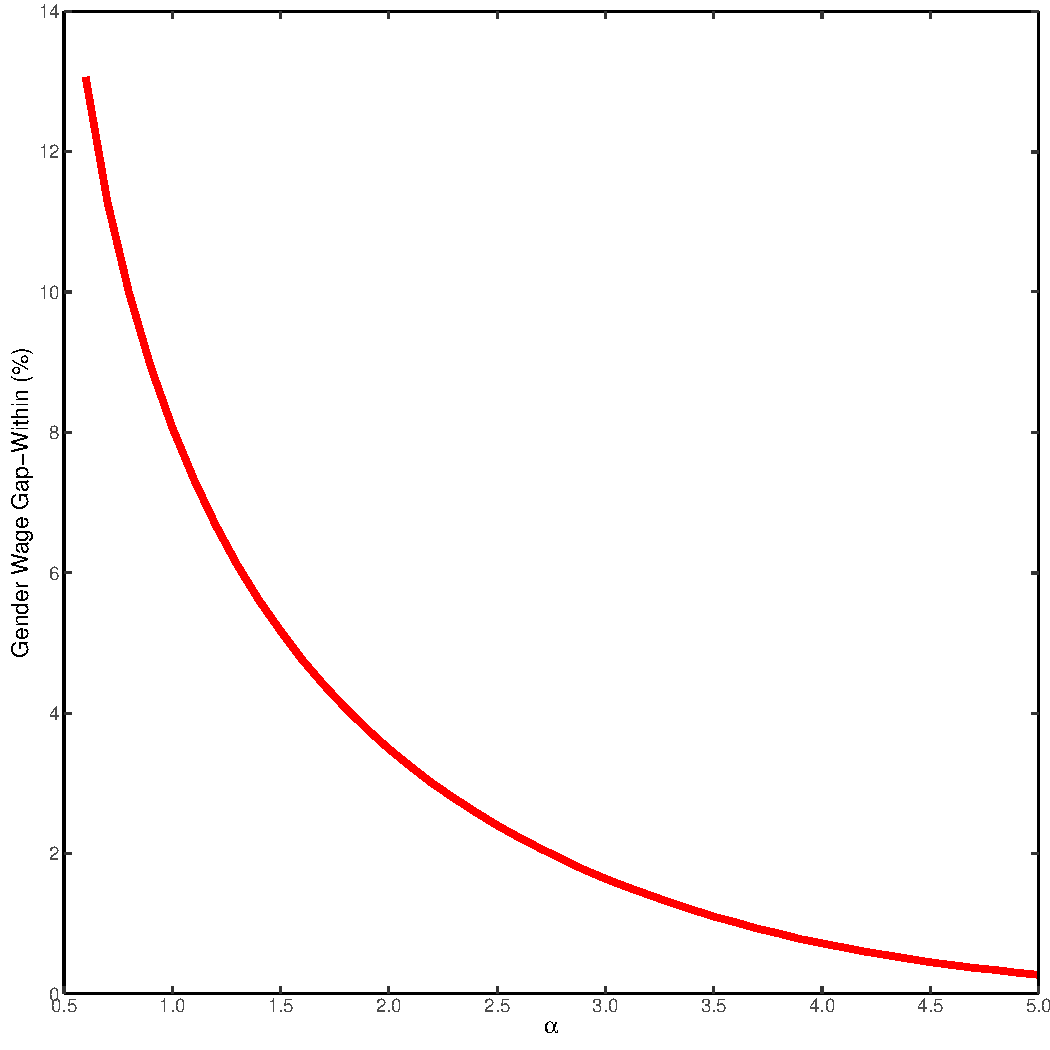
\includegraphics{./figure5.pdf}
\caption{}
\end{center}
\end{figure}
\renewcommand{\thefigure}{6}

\begin{figure}[htb]
\begin{center}
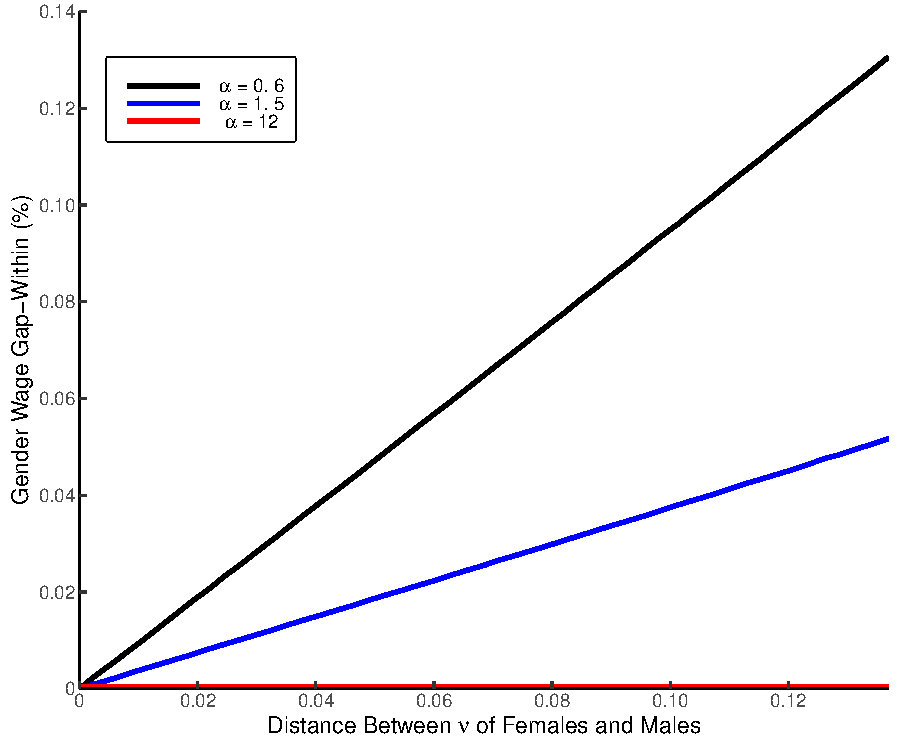
\includegraphics{./figure6.pdf}
\caption{}
\end{center}
\end{figure}

\section{Appendix Tables}

\renewcommand{\thesubsection}{A.\arabic{subsection}}
\setcounter{table}{0}
\renewcommand{\thetable}{A.\arabic{table}}
\begin{table}[ht]
\centering
\caption{A Simple Case with Two-Earner Households
} \label{table7}
\scalebox{0.85}{
\begin{tabular}{lccccccc}  \hline
\\
\footnotesize{
Occupation}          & \footnotesize{$\%$ Workers}&\footnotesize{Bunching Ratio}   &\footnotesize{Earnings}   &\footnotesize{$l_1+l_2$}&  \footnotesize{$l$}   & \footnotesize{$\%$ Females}& \footnotesize{E. Gap}\\ \\
(1)                 & (2)         &       (3)       &  (4)   &(5)      &  (6)   & (7)&(8)\\
\hline\\\\
       \multicolumn{8}{l}{\footnotesize Panel A: Positive Assortative Matching}\\
\hline\\
1              & 67      &  0.65     &  0.19      &   0.77 &  0.73  & 50             & 1.104 \\
2              & 33       &  0.51      &  0.79       &   0.84 &  0.83  & 50          & 1.003\\
 \hline \\
\\
Gender Earnings Gap  &\multicolumn{7}{l}{1.070}\\
\hline \\\\
                      \multicolumn{8}{l}{\footnotesize Panel B: Negative Assortative Matching}\\
\hline\\
1              & 41      &  0.57     &  0.56      &   0.86 &  0.84  & 50             & 1.035 \\
2              & 59       &  0.53      &  0.27       &   0.74 &  0.73  & 50          & 1.013\\
 \hline \\
\\
Gender Earnings Gap  &\multicolumn{7}{l}{1.022}\\
\hline \\\\
                      \multicolumn{8}{l}{\footnotesize Panel C: Observed Assortative Matching}\\
\hline\\
1              & 53      &  0.61     &  0.35      &   0.81 &  0.78  & 50             & 1.059 \\
2              & 47       &  0.51      &  0.45       &   0.81 &  0.80  & 50          & 1.005\\
\\
Gender Earnings Gap  &\multicolumn{7}{l}{1.034}\\
\hline
\\
\multicolumn{8} {p{6.8in}} { {\footnotesize{
}}}
\end{tabular}
}
\end{table}

\renewcommand{\thefigure}{7}

\begin{figure}[htb]
\begin{center}
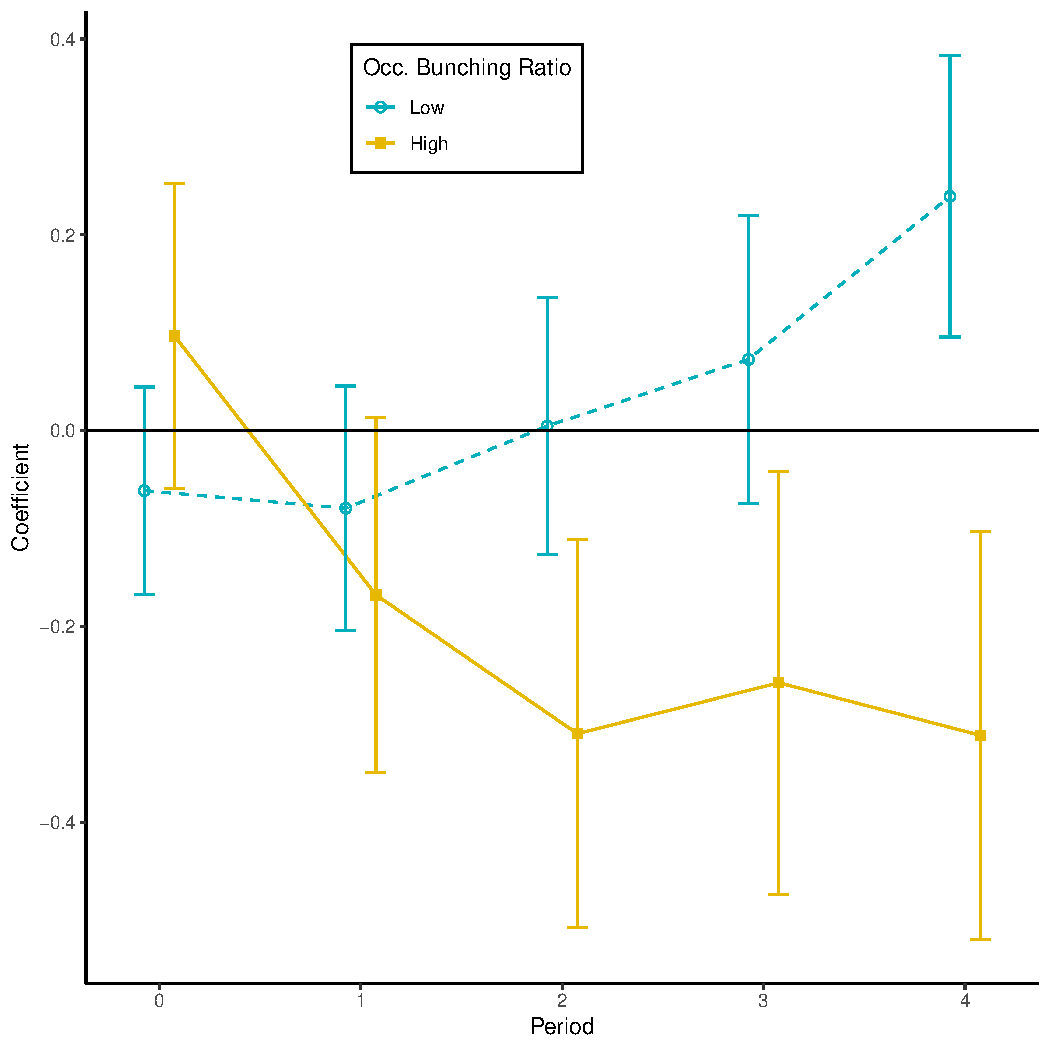
\includegraphics{./psid_penalty.pdf}
\caption{}
\end{center}
\end{figure}

% table with the manual assignment of cnef occupations to soc
% occupations
\def\sep{0.5em}
\def\fns{\footnotesize}
\begin{table}[htpb]\centering
    \caption{Mapping of Occupations: CPS and CNEF-PSID}
    \tiny

\begin{tabular}{llcc}
\hline
   \\[.5em]
ratio8to5 & Occupation CPS &Occupation CNEF-PSID\\[.5em]

\hline
   \\[.5em]

\textbf{Low ratio8to5 Occupations} &                \\[.5em]



0.710  &  (Major group 11)  Healthcare Support &(7) Related Medical Job\\[.5em]
 0.505 & (32)  Musician, Singers and Related Workers &(17) Music/Perform\\[.5em]
 0.734 & (195) Computer Operator                     &(34) Computer Operator\\[.5em]
   0.547    &  (52) Nursing, Psychiatric, and Home Health Aides                                           &(52) HH Supervisor\\[.5em]
 
 0.571  & (64)   Food Cooking, Machine Operators and Tenders        &(53) Cook/Waiter\\[.5em]
 0.767  &  (232) Maid and Housekeeping Cleaners                     &(54) Domestic Help\\[.5em]
 0.624  &  (98)  Janitor and Building Cleaners                      &(55) Janitor\\[.5em]
 0.657  &  (126) Laundry and Dry-Cleaning Workers                   &(56) Dry-Cleaner\\[.5em]
 0.533  &  (42)  Security Guards and Gaming Surveillance Officers   &(58) Security Service\\[.5em]
 0.667   & (Major group 15)  Personal Care and Service              &(59) Service Worker\\[.5em]
 
 0.696  &  (154) Farm, Ranch, and Other Agricultural Managers &(61) Farm Manager\\[.5em]
 0.653 &  (121) Farmers and Ranchers &(62) Farm Hand\\[.5em]
 0.304 &  (7) Fishers and Related Fishing Workers &(64) Fisher/Hunter\\[.5em]

 0.673 &  (134) Inspectors, Testers, Sorters, Samplers, and Weighers &(70) Inspector\\[.5em]
 0.404 &  (14) Derrick, Rotary Drill, and Service Unit Operators, Oil, Gas, and Mining &(71) Miner\\[.5em]
 0.568 &  (62) Chemical Technician &(74) Chemical Worker\\[.5em]

 0.468 &  (22) Shoe and Leather Workers and Repairers &(80) Shoemaker\\[.5em]
 0.663 &  (129) Tool and Die Makers &(83) Tool/Die Maker\\[.5em]
 0.708 & (166)  Broadcast and Sound Engineering Technicians and Radio Operators &(86) Broadcaster\\[.5em]
 0.709 & (170) Jewelers and Precious Stone and Metal Workers &(88) Jewelry Maker\\[.5em]

 0.637 & (111) Transportation Attendants &(98) Transportation Operator\\[.5em]

\textbf{High ratio8to5 Occupations} &   \\[.5em]


 0.825  &    (Major Group 4)  Architecture and Engineering   &(2) Architect/Engineer\\[.5em]
 0.780  & (247) Engineering Technicians, Except Drafters &(3) Enginnering Technician Expert\\[.5em]
 0.830       & (Major Group 7) Life,Physical, and Social Sciences                                                &(5) Life/Physical Science\\[.5em]
 
 0.824  &  (337) Lawyers                                  &(12) Lawyer\\[.5em]
 0.829  &  (353) Elementary and Middle School Teachers  &(13) Educator\\[.5em]
 0.931  &  (480) Library Assistants, Clerical  &(14) Cleric\\[.5em]
 0.760  &  (221) Writers and Authors  &(15) Author\\[.5em]
 0.756  &  (218) Athletes, Coaches, Umpires, and Related Workers  &(18) Professional Athlete\\[.5em]

 0.892 &  (454) Bookkeeping, Accounting, and Auditing Clerks         &(33) Bookkeeper/Cashier\\[.5em]
 0.825 &  (339) Office and Administrative Support Workers, All Other &(39) Office Worker, etc.\\[.5em]

 0.831 &  (355) Other Business Operations Specialists      &(41) Business Operator\\[.5em]
 0.844 &  (385) Parts Salespersons                         &(43) Technical Salesperson\\[.5em]
 0.863 &  (425) Sales and Related Workers, All Other       &(45) Vendor\\[.5em]
 0.785 &  (253) Sales Representatives, Services, All Other &(49) Salesperson\\[.5em]

 0.779  & (246) Cabinetmakers and Bench Carpenters             &(81) Cabinet Maker\\[.5em]
 0.818 &  (346) Pipelayers, Plumbers, Pipefitters, and Steamfitters &(87) Pipe Fitter\\[.5em]
 0.854 &  (405) Glaziers &(89) Glazier\\[.5em]
 
 0.838 & (372) Painters, Construction and Maintenance &(93) Painter\\[.5em]
 0.819 & (327) Carpenters &(95) Briclay/Carpenter\\[.5em]

\hline
\end{tabular}
\end{table}







{
\def\sep{0.6em}
\def\fns{\footnotesize}
\begin{table}[htbp]\centering
\footnotesize
\caption{Regression Child Penalty \label{event_reg}}
\begin{tabular}{l c c c c }
\toprule
                          && All Occs   &  Low $ratio8to5$     & High
                          $ratio8to5$      \tabularnewline[\sep]
$\alpha_[-2,1]$              && -0.002    & -0.061      & 0.097    \tabularnewline
                          &&\fns{(0.05)}&\fns{(0.05)} & \fns{(0.08)} \tabularnewline[\sep]
$\alpha_[2,3]$               && -0.184    & -0.079      & -0.168    \tabularnewline
                          &&\fns{(0.06)}&\fns{(0.06)} & \fns{(0.08)} \tabularnewline[\sep]
$\alpha_[4,5]$               && -0.210    & 0.005      & -0.309    \tabularnewline
                          &&\fns{(0.06)}&\fns{(0.07)} & \fns{(0.10)} \tabularnewline[\sep]
$\alpha_[6,7]$               && -0.251    & 0.073      & -0.257    \tabularnewline
                          &&\fns{(0.07)}&\fns{(0.08)} & \fns{(0.11)} \tabularnewline[\sep]
$\alpha_[8,10]$              && -0.247    & 0.239      & -0.311    \tabularnewline
                          &&\fns{(0.07)}&\fns{(0.07)} & \fns{(0.11)} \tabularnewline[\sep]
		  \bottomrule \tabularnewline
		  \multicolumn{5}{p{4in}}{\setstretch{1.9}\scriptsize{	\emph{Note}: Standard errors in parentheses
}}
\end{tabular}
\end{table}
}


\begin{table}[!htbp]\label{tableA1}
%\begin{table}[h]
\footnotesize

\caption{Classification of ATUS Activities among Routine Care, Enrichment Care, and Other} \label{tableA1}
\def\sym#1{\ifmmode^{#1}\else\(^{#1}\)\fi}
\centering
%\resizebox{\linewidth}{!}{%
\scalebox{0.7}{
\footnotesize{
{\footnotesize{}}%
\begin{tabular}{llcc}

\hline
   \\[.5em]

\textbf{Routine Childcare} &      \\[.5em]



 030101 &   Physical care of household children    \\[.5em]
 030109 &   Looking after children as a primary activity    \\[.5em]
 030301 &  Providing medical care to household children \\[.5em]


\textbf{Enriching childcare (children of all ages)} &      \\[.5em]


030102 &  Reading to/with household children    \\[.5em]
030103 &  Playing with household children, not sports     \\[.5em]
030104 &  Arts and crafts with household children    \\[.5em]
030105 &  Playing sports with household children    \\[.5em]
030106 &  Talking with/listening to household children     \\[.5em]
030107 &  Helping/teaching household children (not related to education)    \\[.5em]
030201 &  Homework (household children)   \\[.5em]
030203  & Home schooling of household children     \\[.5em]


\textbf{Enriching childcare (children ages 2+)} &    \\[.5em]


 1201     & Socializing and communicating  \\[.5em]
120307  &Playing games  \\[.5em]
120309  &Arts and crafts as a hobby  \\[.5em]
120310  &Collecting as a hobby  \\[.5em]
120311  &Hobbies, except arts 8c crafts and collecting \\[.5em]
120401  &Attending performances  \\[.5em]
120402  &Attending museums  \\[.5em]
120403  &Attending movies/films  \\[.5em]
1301     &Participating in sports, exercise, or recreation  \\[.5em]
1302     &Attending sporting/recreational events  \\[.5em]


\textbf{Other childcare} &      \\[.5em]


030108 &Organization and planning for household children  \\[.5em]
030110 &Attending household children's events  \\[.5em]
030111 &Waiting for/with household children  \\[.5em]
030112 &Picking up/dropping off household children  \\[.5em]
030199 &Caring for and helping household children, not elsewhere classified  \\[.5em]
030202 &Meetings and school conferences (household children)  \\[.5em]
030204 &Waiting associated with household children's education  \\[.5em]
030299 &Activities related to household children's education, not elsewhere classified  \\[.5em]
030302 &Obtaining medical care for household children  \\[.5em]
030303 &Waiting associated with household children's health  \\[.5em]
030399 &Activities related to household children's health, not elsewhere classified  \\[.5em]
170301 &Travel related to caring for and helping household children (2003 and 2004) \\[.5em]
180301 &Travel related to caring for and helping household children  \\[.5em]
180302 &Travel related to household children's education  \\[.5em]
180303 &Travel related to household children's health  \\[.5em]
\hline
\multicolumn{3} {p{8.2in}} { {\footnotesize{
Note: These categorizations are used by Stewart (2010). A child must be present during enriching care activities. For children ages 2+, enriching child care
includes leisure activities during which the child was present (see text for further details).
}}}
\end{tabular}{\footnotesize \par}}}
\end{table}
%\end{document}





\begin{table}[!htbp]
\centering{
\caption{Work among Full-time Workers, Married with Children}\label{table1}
\scalebox{0.8}{
\small \begin{tabular}{l*{7}{c}}
\hline
                    &\multicolumn{1}{c}{Weekday}&\multicolumn{1}{c}{Weekend}&\multicolumn{1}{c}{Weekday}&\multicolumn{1}{c}{est4}&\multicolumn{1}{c}{est5}&\multicolumn{1}{c}{est6}\\
\hline
Male Hours Gap PT Spouse Relative to NW Spouse&      -0.121         &     -0.0290         &      -0.104         &      -0.163         &      -0.185         &      -0.247\sym{*}  \\
                    &     (0.116)         &     (0.121)         &     (0.116)         &     (0.117)         &     (0.115)         &     (0.144)         \\
[1em]
Male Hours Gap FT Spouse Relative to NW Spouse&      -0.253\sym{**} &     0.00497         &      -0.249\sym{**} &      -0.269\sym{**} &      -0.245\sym{**} &      -0.160         \\
                    &    (0.0928)         &    (0.0967)         &    (0.0926)         &    (0.0945)         &    (0.0927)         &     (0.114)         \\
\hline
Observations        &        7769         &        7784         &        7769         &        7769         &        7769         &        4766         \\
\hline\hline
                    &\multicolumn{1}{c}{Weekday}&\multicolumn{1}{c}{Weekend}\\
\hline
1                   &       8.040&       2.164\\
                    &            &            \\
[1em]
2                   &       7.919&       2.135\\
                    &            &            \\
[1em]
3                   &       7.788&       2.169\\
                    &            &            \\
[1em]
                    &            &            \\
\hline
Observations        &        7769&        7784\\
\multicolumn{8} {p{7.2in}} { {\footnotesize{
Notes:
Data are from the 2003-2014 American Time Use Surveys (ATUS). The table is based on 18-65 year old ATUS respondents who report working full-time in the activity summary file.  We keep those who are married with spouse present and have at least one own child in the household. The dependent variable is total hours spent on ``work and work-related activities'' on the diary day. Each column reports the coefficient on the ``female'' dummy. Column (5) controls for usual weekly hours worked reported in the activity summary file. Column (6) only includes workers who reported usual weekly hours of less than 50. Individual observations are weighted by ATUS weights for multi-year data files.
}}}
\end{tabular}
}}
\end{table}

\begin{table}[!htbp]
\centering{
\caption{Household Care among Full-time Workers, Married with Children}\label{table1}
\scalebox{0.8}{
\small \begin{tabular}{l*{7}{c}}
\hline
                    &\multicolumn{1}{c}{Weekday}&\multicolumn{1}{c}{Weekend}&\multicolumn{1}{c}{Weekday}&\multicolumn{1}{c}{est4}&\multicolumn{1}{c}{est5}&\multicolumn{1}{c}{est6}\\
\hline
Male Hours Gap PT Spouse Relative to NW Spouse&      0.0702         &      0.0642         &      0.0739\sym{*}  &      0.0885\sym{**} &      0.0925\sym{**} &      0.0650         \\
                    &    (0.0429)         &    (0.0551)         &    (0.0429)         &    (0.0424)         &    (0.0422)         &    (0.0594)         \\
[1em]
Male Hours Gap FT Spouse Relative to NW Spouse&      0.0715\sym{**} &      -0.103\sym{**} &      0.0707\sym{**} &       0.112\sym{***}&       0.108\sym{**} &       0.115\sym{**} \\
                    &    (0.0342)         &    (0.0439)         &    (0.0342)         &    (0.0341)         &    (0.0339)         &    (0.0469)         \\
\hline
Observations        &        7769         &        7784         &        7769         &        7769         &        7769         &        4766         \\
\hline\hline
                    &\multicolumn{1}{c}{Weekday}&\multicolumn{1}{c}{Weekend}\\
\hline
1                   &       0.776&       1.036\\
                    &            &            \\
[1em]
2                   &       0.846&       1.101\\
                    &            &            \\
[1em]
3                   &       0.847&       0.934\\
                    &            &            \\
[1em]
                    &            &            \\
\hline
Observations        &        7769&        7784\\
\multicolumn{8} {p{7.2in}} { {\footnotesize{
Notes:
Data are from the 2003-2014 American Time Use Surveys (ATUS). The table is based on 18-65 year old ATUS respondents who report working full-time in the activity summary file.  We keep those who are married with spouse present and have at least one own child in the household. The dependent variable is total hours spent on ``work and work-related activities'' on the diary day. Each column reports the coefficient on the ``female'' dummy. Column (5) controls for usual weekly hours worked reported in the activity summary file. Column (6) only includes workers who reported usual weekly hours of less than 50. Individual observations are weighted by ATUS weights for multi-year data files.
}}}
\end{tabular}
}}
\end{table}


\clearpage
{
\tiny
\begin{longtable}{llcccc}

\caption{Ratio8to5 by Occupation}\label{tableA4}

\tabularnewline
 & {\tiny{}Occupations}  & {\tiny{}\# FT Workers} & {\tiny{}ratio8to5} & {\tiny{}ratio8to5\_Std}& {\tiny{}\% Females} \tabularnewline
\hline

\endfirsthead

 & {\tiny{}Occupations}  & {\tiny{}\# FT Workers}
& {\tiny{}ratio8to5} & {\tiny{}ratio8to5\_Std}& {\tiny{}\% Females} \tabularnewline

\hline
\endhead

\hline
\multicolumn{6}{c}{{Continued on next page}}

\endfoot
\endlastfoot
 1 & Tank Car, Truck, and Ship Loaders & 5 & 0.000 & -4.979 & 0.000 \\
 2 & Miscellaneous Mathematical Science Occupations & 2 & 0.000 & -4.979 & 0.000 \\
 3 & Media and Communication Equipment Workers, All Other & 1 & 0.000 & -4.979 & 1.000 \\
 4 & Textile Bleaching and Dyeing Machine Operators and Tenders & 2 & 0.092 & -4.360 & 0.370 \\
 5 & Food Preparation and Serving Related Workers, All Other & 2 & 0.160 & -3.898 & 0.523 \\
 6 & Postal Service Mail Sorters, Processors, and Processing Machine Operators & 55 & 0.243 & -3.336 & 0.474 \\
 7 & Fishers and Related Fishing Workers & 7 & 0.304 & -2.927 & 0.087 \\
 8 & Plating and Coating Machine Setters, Operators, and Tenders, Metal and Plastic & 11 & 0.319 & -2.823 & 0.000 \\
 9 & Electrical and Electronics Repairers, Industrial and Utility  & 8 & 0.328 & -2.765 & 0.000 \\
 10 & Locomotive Engineers and Operators & 25 & 0.340 & -2.685 & 0.012 \\
 11 & Railroad Brake, Signal, and Switch Operators & 7 & 0.340 & -2.680 & 0.000 \\
 12 & Extruding and Drawing Machine Setters, Operators, and Tenders, Metal and Plastic & 7 & 0.384 & -2.386 & 0.000 \\
 13 & Bartenders & 83 & 0.401 & -2.271 & 0.573 \\
 14 & Derrick, Rotary Drill, and Service Unit Operators, Oil, Gas, and Mining & 17 & 0.404 & -2.247 & 0.000 \\
 15 & Ushers, Lobby Attendants, and Ticket Takers & 2 & 0.423 & -2.121 & 0.504 \\
 16 & Metal Furnace and Kiln Operators and Tenders & 12 & 0.431 & -2.065 & 0.000 \\
 17 & Motion Picture Projectionists & 1 & 0.432 & -2.063 & 0.000 \\
 18 & Door-to-Door Sales Workers, News and Street Vendors, and Related Workers & 39 & 0.437 & -2.026 & 0.778 \\
 19 & Paper Goods Machine Setters, Operators, and Tenders & 27 & 0.438 & -2.019 & 0.326 \\
 20 & Gaming Services Workers & 37 & 0.455 & -1.906 & 0.596 \\
 21 & Respiratory Therapists & 72 & 0.467 & -1.825 & 0.496 \\
 22 & Shoe and Leather Workers and Repairers & 4 & 0.468 & -1.816 & 0.000 \\
 23 & Material Moving Workers, All Other & 17 & 0.473 & -1.786 & 0.059 \\
 24 & Residential Advisors & 21 & 0.473 & -1.785 & 0.774 \\
 25 & Food and Tobacco Roasting, Baking, and Drying Machine Operators and Tenders & 8 & 0.478 & -1.749 & 0.279 \\
 26 & Tool Grinders, Filers, and Sharpeners & 9 & 0.481 & -1.727 & 0.000 \\
 27 & Emergency Medical Technicians and Paramedics & 72 & 0.484 & -1.709 & 0.221 \\
 28 & Bailiffs, Correctional Officers, and Jailers & 245 & 0.484 & -1.706 & 0.209 \\
 29 & Cutting, Punching, and Press Machine Setters, Operators, and Tenders, Metal and Plastic & 67 & 0.492 & -1.656 & 0.197 \\
 30 & Service Station Attendants & 31 & 0.493 & -1.651 & 0.165 \\
 31 & Fire Fighters & 160 & 0.494 & -1.641 & 0.038 \\
 32 & Musicians, Singers, and Related Workers & 52 & 0.505 & -1.565 & 0.225 \\
 33 & Manufactured Building and Mobile Home Installers & 5 & 0.511 & -1.526 & 0.293 \\
 34 & Molders and Molding Machine Setters, Operators, and Tenders, Metal and Plastic & 30 & 0.517 & -1.484 & 0.266 \\
 35 & Agricultural and Food Science Technicians & 15 & 0.518 & -1.480 & 0.357 \\
 36 & Mining Machine Operators & 27 & 0.518 & -1.478 & 0.015 \\
 37 & Maintenance Workers, Machinery & 29 & 0.519 & -1.471 & 0.019 \\
 38 & Helpers--Extraction Workers & 7 & 0.520 & -1.469 & 0.000 \\
 39 & Electronic Equipment Installers and Repairers, Motor Vehicles & 17 & 0.524 & -1.437 & 0.000 \\
 40 & Hotel, Motel, and Resort Desk Clerks & 38 & 0.530 & -1.398 & 0.776 \\
 41 & Logging Workers & 28 & 0.533 & -1.381 & 0.000 \\
 42 & Security Guards and Gaming Surveillance Officers  & 350 & 0.533 & -1.378 & 0.181 \\
 43 & Bridge and Lock Tenders & 2 & 0.533 & -1.377 & 0.404 \\
 44 & Dispatchers & 129 & 0.536 & -1.357 & 0.403 \\
 45 & Police and Sheriff's Patrol Officers & 392 & 0.536 & -1.356 & 0.111 \\
 46 & Communications Equipment Operators, All Other & 6 & 0.539 & -1.339 & 0.755 \\
 47 & Lay-Out Workers, Metal and Plastic & 4 & 0.540 & -1.333 & 0.000 \\
 48 & Postal Service Clerks & 94 & 0.540 & -1.331 & 0.422 \\
 49 & Miscellaneous Plant and System Operators & 18 & 0.540 & -1.328 & 0.196 \\
 50 & Supervisors, Protective Service Workers, All Other & 49 & 0.542 & -1.314 & 0.185 \\
 51 & Stationary Engineers and Boiler Operators & 63 & 0.546 & -1.292 & 0.062 \\
 52 & Nursing, Psychiatric, and Home Health Aides & 810 & 0.547 & -1.284 & 0.881 \\
 53 & Crushing, Grinding, Polishing, Mixing, and Blending Workers  & 48 & 0.549 & -1.270 & 0.046 \\
 54 & Taxi Drivers and Chauffeurs & 122 & 0.552 & -1.252 & 0.193 \\
 55 & First-Line Supervisors/Managers of Fire Fighting and Prevention Workers & 37 & 0.558 & -1.210 & 0.038 \\
 56 & Cleaning, Washing, and Metal Pickling Equipment Operators and Tenders & 5 & 0.559 & -1.204 & 0.267 \\
 57 & Personal and Home Care Aides & 264 & 0.560 & -1.197 & 0.819 \\
 58 & Dining Room and Cafeteria Attendants and Bartender Helpers & 55 & 0.560 & -1.194 & 0.504 \\
 59 & Forging Machine Setters, Operators, and Tenders, Metal and Plastic & 4 & 0.566 & -1.158 & 0.000 \\
 60 & Statistical Assistants & 14 & 0.567 & -1.151 & 0.555 \\
 61 & Waiters and Waitresses & 282 & 0.568 & -1.141 & 0.734 \\
 62 & Chemical Technicians & 41 & 0.568 & -1.140 & 0.172 \\
 63 & Bakers & 63 & 0.571 & -1.121 & 0.465 \\
 64 & Food Cooking Machine Operators and Tenders & 18 & 0.571 & -1.120 & 0.448 \\
 65 & Dishwashers & 55 & 0.575 & -1.093 & 0.265 \\
 66 & Tire Builders & 14 & 0.580 & -1.060 & 0.100 \\
 67 & Baggage Porters, Bellhops, and Concierges & 32 & 0.582 & -1.049 & 0.098 \\
 68 & Packaging and Filling Machine Operators and Tenders & 141 & 0.582 & -1.043 & 0.473 \\
 69 & First-Line Supervisors/Managers of Police and Detectives & 85 & 0.585 & -1.027 & 0.226 \\
 70 & Food Servers, Nonrestaurant & 48 & 0.587 & -1.012 & 0.512 \\
 71 & Metal Workers and Plastic Workers, All Other & 226 & 0.587 & -1.011 & 0.187 \\
 72 & Boilermakers & 11 & 0.587 & -1.010 & 0.000 \\
 73 & Biological Technicians & 14 & 0.591 & -0.989 & 0.399 \\
 74 & Ship and Boat Captains and Operators & 11 & 0.592 & -0.980 & 0.070 \\
 75 & Industrial Truck and Tractor Operators & 290 & 0.594 & -0.965 & 0.045 \\
 76 & Production Workers, All Other & 471 & 0.596 & -0.949 & 0.388 \\
 77 & First-Line Supervisors/Managers of Food Preparation and Serving Workers & 241 & 0.597 & -0.947 & 0.642 \\
 78 & Stock Clerks and Order Fillers & 489 & 0.598 & -0.942 & 0.445 \\
 79 & Hosts and Hostesses, Restaurant, Lounge, and Coffee Shop & 17 & 0.598 & -0.936 & 0.945 \\
 80 & Machine Feeders and Offbearers & 21 & 0.599 & -0.933 & 0.420 \\
 81 & Air Traffic Controllers and Airfield Operations Specialists & 29 & 0.599 & -0.929 & 0.241 \\
 82 & Food Service Managers & 417 & 0.600 & -0.928 & 0.432 \\
 83 & Gaming Cage Workers & 7 & 0.600 & -0.925 & 0.879 \\
 84 & Aircraft Mechanics and Service Technicians & 71 & 0.600 & -0.922 & 0.020 \\
 85 & Printing Machine Operators & 93 & 0.606 & -0.883 & 0.134 \\
 86 & Railroad Conductors and Yardmasters & 29 & 0.607 & -0.875 & 0.030 \\
 87 & Heat Treating Equipment Setters, Operators, and Tenders, Metal and Plastic & 2 & 0.611 & -0.853 & 0.000 \\
 88 & Counter Attendants, Cafeteria, Food Concession, and Coffee Shop & 26 & 0.612 & -0.842 & 0.676 \\
 89 & Aircraft Structure, Surfaces, Rigging, and Systems Assemblers & 10 & 0.613 & -0.839 & 0.453 \\
 90 & Motor Vehicle Operators, All Other & 12 & 0.616 & -0.815 & 0.222 \\
 91 & Engine and Other Machine Assemblers & 13 & 0.618 & -0.807 & 0.119 \\
 92 & Helpers, Construction Trades & 32 & 0.619 & -0.795 & 0.029 \\
 93 & Cashiers & 566 & 0.621 & -0.781 & 0.778 \\
 94 & Electrical, Electronics, and Electromechanical Assemblers & 90 & 0.622 & -0.775 & 0.515 \\
 95 & Machinists & 200 & 0.622 & -0.774 & 0.059 \\
 96 & Miscellaneous Entertainment Attendants and Related Workers & 33 & 0.623 & -0.770 & 0.516 \\
 97 & Coin, Vending, and Amusement Machine Servicers and Repairers & 26 & 0.623 & -0.770 & 0.203 \\
 98 & Janitors and Building Cleaners & 821 & 0.624 & -0.761 & 0.275 \\
 99 & Milling and Planing Machine Setters, Operators, and Tenders, Metal and Plastic & 2 & 0.625 & -0.756 & 0.000 \\
 100 & Cooks & 524 & 0.627 & -0.743 & 0.403 \\
 101 & Telemarketers & 35 & 0.627 & -0.742 & 0.642 \\
 102 & Parking Lot Attendants & 24 & 0.629 & -0.728 & 0.032 \\
 103 & Lathe and Turning Machine Tool Setters, Operators, and Tenders, Metal and Plastic & 12 & 0.630 & -0.725 & 0.081 \\
 104 & Telephone Operators & 27 & 0.630 & -0.724 & 0.655 \\
 105 & First-line Supervisors/Managers of Gaming Workers & 64 & 0.630 & -0.723 & 0.297 \\
 106 & Registered Nurses & 1369 & 0.633 & -0.701 & 0.912 \\
 107 & Health Diagnosing and Treating Practitioners, All Other & 3 & 0.634 & -0.694 & 0.596 \\
 108 & Laborers and Freight, Stock, and Material Movers, Hand & 641 & 0.634 & -0.693 & 0.166 \\
 109 & Miscellaneous Assemblers and Fabricators & 462 & 0.635 & -0.691 & 0.371 \\
 110 & Prepress Technicians and Workers & 20 & 0.637 & -0.677 & 0.607 \\
 111 & Transportation Attendants & 26 & 0.637 & -0.674 & 0.529 \\
 112 & Structural Iron and Steel Workers & 34 & 0.639 & -0.663 & 0.000 \\
 113 & Reservation and Transportation Ticket Agents and Travel Clerks & 55 & 0.639 & -0.663 & 0.600 \\
 114 & Grinding, Lapping, Polishing, and Buffing Machine Tool Setters, Operators, and Tenders, Metal and Plastic & 22 & 0.641 & -0.650 & 0.304 \\
 115 & Extruding, Forming, Pressing, and Compacting Machine Setters, Operators, and Tenders & 17 & 0.642 & -0.639 & 0.146 \\
 116 & Chemical Processing Machine Setters, Operators, and Tenders & 34 & 0.645 & -0.621 & 0.181 \\
 117 & Cutting Workers & 49 & 0.645 & -0.620 & 0.241 \\
 118 & First-Line Supervisors/Managers of Production and Operating Workers & 499 & 0.650 & -0.590 & 0.194 \\
 119 & Cooling and Freezing Equipment Operators and Tenders & 2 & 0.650 & -0.587 & 0.000 \\
 120 & Textile, Apparel, and Furnishings Workers, All Other & 12 & 0.651 & -0.583 & 0.461 \\
 121 & Farmers and Ranchers & 217 & 0.653 & -0.566 & 0.328 \\
 122 & Cleaners of Vehicles and Equipment & 118 & 0.654 & -0.564 & 0.165 \\
 123 & Packers and Packagers, Hand & 184 & 0.655 & -0.556 & 0.505 \\
 124 & Office Machine Operators, Except Computer & 18 & 0.657 & -0.542 & 0.627 \\
 125 & Industrial and Refractory Machinery Mechanics & 262 & 0.657 & -0.542 & 0.025 \\
 126 & Laundry and Dry-Cleaning Workers & 81 & 0.657 & -0.542 & 0.609 \\
 127 & Food Batchmakers & 44 & 0.658 & -0.531 & 0.593 \\
 128 & Bus Drivers & 181 & 0.662 & -0.505 & 0.569 \\
 129 & Tool and Die Makers & 49 & 0.663 & -0.501 & 0.012 \\
 130 & Photographers & 57 & 0.664 & -0.493 & 0.401 \\
 131 & Signal and Track Switch Repairers & 3 & 0.668 & -0.463 & 0.000 \\
 132 & Graders and Sorters, Agricultural Products & 49 & 0.670 & -0.450 & 0.677 \\
 133 & Driver/Sales Workers and Truck Drivers & 1420 & 0.672 & -0.436 & 0.060 \\
 134 & Inspectors, Testers, Sorters, Samplers, and Weighers & 382 & 0.673 & -0.434 & 0.395 \\
 135 & Miscellaneous Agricultural Workers & 340 & 0.673 & -0.429 & 0.194 \\
 136 & Clinical Laboratory Technologists and Technicians & 183 & 0.674 & -0.426 & 0.729 \\
 137 & Refuse and Recyclable Material Collectors & 36 & 0.674 & -0.425 & 0.043 \\
 138 & Textile Winding, Twisting, and Drawing Out Machine Setters, Operators, and Tenders & 11 & 0.678 & -0.395 & 0.421 \\
 139 & Licensed Practical and Licensed Vocational Nurses & 252 & 0.682 & -0.374 & 0.911 \\
 140 & Chefs and Head Cooks & 115 & 0.682 & -0.370 & 0.194 \\
 141 & Animal Breeders & 1 & 0.684 & -0.356 & 0.000 \\
 142 & Lodging Managers & 75 & 0.685 & -0.351 & 0.534 \\
 143 & Food Preparation Workers & 161 & 0.686 & -0.345 & 0.600 \\
 144 & Shipping, Receiving, and Traffic Clerks & 267 & 0.686 & -0.341 & 0.305 \\
 145 & Other Life, Physical, and Social Science Technicians & 56 & 0.688 & -0.332 & 0.555 \\
 146 & Other Extraction Workers & 22 & 0.688 & -0.328 & 0.014 \\
 147 & Clergy & 231 & 0.690 & -0.317 & 0.189 \\
 148 & Crane and Tower Operators & 21 & 0.690 & -0.316 & 0.064 \\
 149 & Crossing Guards & 15 & 0.693 & -0.299 & 0.521 \\
 150 & Pile-Driver Operators & 1 & 0.694 & -0.291 & 0.000 \\
 151 & Supervisors, Transportation and Material Moving Workers & 121 & 0.694 & -0.288 & 0.206 \\
 152 & Weighers, Measurers, Checkers, and Samplers, Recordkeeping & 43 & 0.694 & -0.287 & 0.398 \\
 153 & Drilling and Boring Machine Tool Setters, Operators, and Tenders, Metal and Plastic & 4 & 0.695 & -0.284 & 0.000 \\
 154 & Farm, Ranch, and Other Agricultural Managers & 163 & 0.696 & -0.279 & 0.173 \\
 155 & Optometrists & 15 & 0.698 & -0.263 & 0.306 \\
 156 & Couriers and Messengers & 94 & 0.700 & -0.252 & 0.153 \\
 157 & Petroleum Engineers & 14 & 0.700 & -0.247 & 0.107 \\
 158 & Transportation Inspectors & 18 & 0.701 & -0.245 & 0.227 \\
 159 & Bus and Truck Mechanics and Diesel Engine Specialists & 174 & 0.701 & -0.243 & 0.004 \\
 160 & Rolling Machine Setters, Operators, and Tenders, Metal and Plastic & 10 & 0.701 & -0.243 & 0.129 \\
 161 & Religious Workers, All Other & 37 & 0.703 & -0.232 & 0.683 \\
 162 & Gaming Managers & 16 & 0.704 & -0.225 & 0.219 \\
 163 & Podiatrists & 6 & 0.704 & -0.221 & 0.000 \\
 164 & Agricultural Inspectors & 9 & 0.705 & -0.214 & 0.318 \\
 165 & First-Line Supervisors/Managers of Correctional Officers & 24 & 0.707 & -0.204 & 0.309 \\
 166 & Broadcast and Sound Engineering Technicians and Radio Operators & 37 & 0.708 & -0.198 & 0.093 \\
 167 & Announcers & 22 & 0.708 & -0.195 & 0.380 \\
 168 & First-Line Supervisors/Managers of Housekeeping and Janitorial Workers & 123 & 0.708 & -0.193 & 0.443 \\
 169 & Heavy Vehicle and Mobile Equipment Service Technicians and Mechanics & 117 & 0.709 & -0.189 & 0.008 \\
 170 & Jewelers and Precious Stone and Metal Workers & 20 & 0.709 & -0.188 & 0.514 \\
 171 & Geological and Petroleum Technicians & 11 & 0.709 & -0.186 & 0.381 \\
 172 & Recreation and Fitness Workers & 101 & 0.710 & -0.184 & 0.675 \\
 173 & Marine Engineers and Naval Architects & 6 & 0.711 & -0.173 & 0.000 \\
 174 & Helpers--Production Workers & 23 & 0.711 & -0.172 & 0.266 \\
 175 & Aircraft Pilots and Flight Engineers & 51 & 0.713 & -0.161 & 0.035 \\
 176 & Avionics Technicians & 8 & 0.713 & -0.161 & 0.063 \\
 177 & Combined Food Preparation and Serving Workers, Including Fast Food & 60 & 0.714 & -0.152 & 0.639 \\
 178 & Entertainers and Performers, Sports and Related Workers, All Other & 9 & 0.715 & -0.151 & 0.507 \\
 179 & Ambulance Drivers and Attendants, Except Emergency Medical Technicians & 4 & 0.719 & -0.124 & 0.000 \\
 180 & Personal Care and Service Workers, All Other & 27 & 0.720 & -0.116 & 0.524 \\
 181 & Millwrights & 34 & 0.720 & -0.112 & 0.007 \\
 182 & Dancers and Choreographers & 5 & 0.720 & -0.112 & 0.667 \\
 183 & Power Plant Operators, Distributors, and Dispatchers & 24 & 0.724 & -0.088 & 0.066 \\
 184 & Butchers and Other Meat, Poultry, and Fish Processing Workers & 123 & 0.725 & -0.081 & 0.253 \\
 185 & Sawing Machine Setters, Operators, and Tenders, Wood & 20 & 0.725 & -0.079 & 0.020 \\
 186 & Water and Liquid Waste Treatment Plant and System Operators & 52 & 0.728 & -0.058 & 0.094 \\
 187 & Woodworking Machine Setters, Operators, and Tenders, Except Sawing & 21 & 0.729 & -0.057 & 0.376 \\
 188 & Materials Engineers & 24 & 0.730 & -0.046 & 0.106 \\
 189 & Massage Therapists & 25 & 0.730 & -0.046 & 0.883 \\
 190 & Textile Knitting and Weaving Machine Setters, Operators, and Tenders & 4 & 0.731 & -0.038 & 0.503 \\
 191 & Septic Tank Servicers and Sewer Pipe Cleaners & 6 & 0.732 & -0.034 & 0.000 \\
 192 & Animal Trainers & 16 & 0.733 & -0.029 & 0.469 \\
 193 & Explosives Workers, Ordnance Handling Experts, and Blasters & 3 & 0.733 & -0.025 & 0.000 \\
 194 & Operating Engineers and Other Construction Equipment Operators & 217 & 0.734 & -0.023 & 0.025 \\
 195 & Computer Operators & 85 & 0.734 & -0.018 & 0.411 \\
 196 & Painting Workers & 87 & 0.734 & -0.016 & 0.107 \\
 197 & Physicians and Surgeons & 503 & 0.735 & -0.010 & 0.313 \\
 198 & Tailors, Dressmakers, and Sewers & 34 & 0.736 & -0.008 & 0.871 \\
 199 & Biomedical Engineers & 7 & 0.736 & -0.005 & 0.000 \\
 200 & Other Transportation Workers & 5 & 0.736 & -0.003 & 0.040 \\
 201 & Editors & 105 & 0.737 & -0.001 & 0.549 \\
 202 & Paving, Surfacing, and Tamping Equipment Operators & 10 & 0.737 & 0.004 & 0.000 \\
 203 & Nuclear Engineers & 7 & 0.739 & 0.011 & 0.000 \\
 204 & Sheet Metal Workers & 73 & 0.739 & 0.012 & 0.029 \\
 205 & Television, Video, and Motion Picture Camera Operators and Editors & 17 & 0.739 & 0.016 & 0.032 \\
 206 & First-Line Supervisors/Managers of Retail Sales Workers & 1575 & 0.740 & 0.018 & 0.409 \\
 207 & First-Line Supervisors/Managers of Farming, Fishing, and Forestry Workers & 31 & 0.741 & 0.029 & 0.076 \\
 208 & Pumping Station Operators & 12 & 0.744 & 0.047 & 0.000 \\
 209 & Molders, Shapers, and Casters, Except Metal and Plastic & 14 & 0.744 & 0.049 & 0.401 \\
 210 & Structural Metal Fabricators and Fitters & 7 & 0.745 & 0.052 & 0.000 \\
 211 & Health Diagnosing and Treating Practitioner Support Technicians & 204 & 0.746 & 0.062 & 0.798 \\
 212 & Counter and Rental Clerks & 45 & 0.749 & 0.079 & 0.366 \\
 213 & Producers and Directors & 89 & 0.749 & 0.085 & 0.341 \\
 214 & Electrical Power-Line Installers and Repairers & 74 & 0.750 & 0.086 & 0.008 \\
 215 & Computer Control Programmers and Operators & 33 & 0.751 & 0.098 & 0.009 \\
 216 & Welding, Soldering, and Brazing Workers & 276 & 0.752 & 0.103 & 0.028 \\
 217 & Cementing and Gluing Machine Operators and Tenders & 7 & 0.755 & 0.119 & 0.532 \\
 218 & Athletes, Coaches, Umpires, and Related Workers & 72 & 0.756 & 0.131 & 0.457 \\
 219 & Diagnostic Related Technologists and Technicians & 144 & 0.759 & 0.147 & 0.735 \\
 220 & Computer Support Specialists & 229 & 0.759 & 0.150 & 0.242 \\
 221 & Writers and Authors & 82 & 0.760 & 0.157 & 0.526 \\
 222 & Semiconductor Processors & 2 & 0.760 & 0.158 & 0.318 \\
 223 & News Analysts, Reporters and Correspondents & 58 & 0.760 & 0.159 & 0.454 \\
 224 & Hazardous Materials Removal Workers & 11 & 0.761 & 0.164 & 0.233 \\
 225 & Other Teachers and Instructors & 238 & 0.762 & 0.167 & 0.623 \\
 226 & Administrative Services Managers & 64 & 0.762 & 0.168 & 0.351 \\
 227 & Artists and Related Workers & 68 & 0.765 & 0.189 & 0.545 \\
 228 & Postsecondary Teachers & 669 & 0.765 & 0.190 & 0.458 \\
 229 & Conveyor Operators and Tenders & 4 & 0.766 & 0.197 & 0.050 \\
 230 & Sales Engineers & 29 & 0.767 & 0.205 & 0.134 \\
 231 & Dredge, Excavating, and Loading Machine Operators & 31 & 0.767 & 0.206 & 0.004 \\
 232 & Maids and Housekeeping Cleaners & 435 & 0.767 & 0.206 & 0.914 \\
 233 & Electric Motor, Power Tool, and Related Repairers & 26 & 0.768 & 0.209 & 0.082 \\
 234 & Pharmacists & 110 & 0.768 & 0.210 & 0.469 \\
 235 & Highway Maintenance Workers & 67 & 0.768 & 0.210 & 0.005 \\
 236 & Logisticians & 38 & 0.768 & 0.212 & 0.322 \\
 237 & Switchboard Operators, Including Answering Service & 13 & 0.768 & 0.213 & 0.676 \\
 238 & First-Line Supervisors/Managers of Landscaping, Lawn Service, and Groundskeeping Workers & 124 & 0.769 & 0.219 & 0.041 \\
 239 & Retail Salespersons & 831 & 0.774 & 0.253 & 0.514 \\
 240 & Order Clerks & 58 & 0.775 & 0.260 & 0.583 \\
 241 & Roofers & 60 & 0.776 & 0.261 & 0.012 \\
 242 & Commercial Divers & 3 & 0.777 & 0.271 & 0.000 \\
 243 & Directors, Religious Activities and Education & 36 & 0.777 & 0.271 & 0.485 \\
 244 & First-Line Supervisors/Managers of Construction Trades and Extraction Workers & 421 & 0.777 & 0.272 & 0.039 \\
 245 & Secondary School Teachers & 728 & 0.778 & 0.277 & 0.573 \\
 246 & Cabinetmakers and Bench Carpenters & 36 & 0.779 & 0.282 & 0.043 \\
 247 & Engineering Technicians, Except Drafters & 232 & 0.780 & 0.288 & 0.181 \\
 248 & Tax Preparers & 30 & 0.781 & 0.295 & 0.618 \\
 249 & General and Operations Managers & 604 & 0.781 & 0.298 & 0.328 \\
 250 & First-Line Supervisors/Managers of Mechanics, Installers, and Repairers & 212 & 0.782 & 0.304 & 0.065 \\
 251 & Animal Control Workers & 6 & 0.783 & 0.314 & 0.375 \\
 252 & Aerospace Engineers & 55 & 0.784 & 0.318 & 0.202 \\
 253 & Sales Representatives, Services, All Other & 265 & 0.785 & 0.322 & 0.320 \\
 254 & Industrial Production Managers & 181 & 0.785 & 0.323 & 0.153 \\
 255 & Construction Managers & 464 & 0.786 & 0.332 & 0.046 \\
 256 & Riggers & 5 & 0.787 & 0.338 & 0.000 \\
 257 & Child Care Workers & 446 & 0.787 & 0.338 & 0.940 \\
 258 & Chiropractors & 30 & 0.789 & 0.354 & 0.264 \\
 259 & Other Installation, Maintenance, and Repair Workers & 86 & 0.790 & 0.357 & 0.067 \\
 260 & Sailors and Marine Oilers & 6 & 0.790 & 0.359 & 0.266 \\
 261 & Conservation Scientists and Foresters & 15 & 0.791 & 0.365 & 0.256 \\
 262 & First-Line Supervisors/Managers of Office and Administrative Support Workers & 905 & 0.791 & 0.367 & 0.682 \\
 263 & Miscellaneous Health Technologists and Technicians & 59 & 0.792 & 0.370 & 0.620 \\
 264 & Chief Executives & 922 & 0.792 & 0.373 & 0.287 \\
 265 & Real Estate Brokers and Sales Agents & 361 & 0.793 & 0.378 & 0.584 \\
 266 & Construction Laborers & 434 & 0.793 & 0.378 & 0.040 \\
 267 & First-Line Supervisors/Managers of Non-Retail Sales Workers & 681 & 0.793 & 0.382 & 0.274 \\
 268 & Sewing Machine Operators & 102 & 0.794 & 0.384 & 0.717 \\
 269 & Nonfarm Animal Caretakers & 60 & 0.794 & 0.389 & 0.734 \\
 270 & Managers, All Other & 2083 & 0.795 & 0.391 & 0.346 \\
 271 & Shoe Machine Operators and Tenders & 1 & 0.795 & 0.392 & 1.000 \\
 272 & Computer Scientists and Systems Analysts & 462 & 0.796 & 0.396 & 0.270 \\
 273 & Mail Clerks and Mail Machine Operators, Except Postal Service & 52 & 0.796 & 0.396 & 0.477 \\
 274 & Electricians & 420 & 0.796 & 0.398 & 0.015 \\
 275 & Payroll and Timekeeping Clerks & 103 & 0.797 & 0.406 & 0.898 \\
 276 & Transportation, Storage, and Distribution Managers & 157 & 0.798 & 0.410 & 0.170 \\
 277 & Physician Assistants & 46 & 0.798 & 0.411 & 0.774 \\
 278 & Miscellaneous Personal Appearance Workers & 57 & 0.799 & 0.421 & 0.935 \\
 279 & Database Administrators & 69 & 0.799 & 0.422 & 0.358 \\
 280 & Architects, Except Naval & 118 & 0.800 & 0.426 & 0.241 \\
 281 & Roustabouts, Oil and Gas & 2 & 0.800 & 0.426 & 0.000 \\
 282 & Tax Examiners, Collectors, and Revenue Agents & 44 & 0.801 & 0.434 & 0.387 \\
 283 & Maintenance and Repair Workers, General & 203 & 0.802 & 0.437 & 0.040 \\
 284 & Agents and Business Managers of Artists, Performers, and Athletes & 20 & 0.803 & 0.446 & 0.233 \\
 285 & Fish and Game Wardens & 2 & 0.803 & 0.448 & 0.000 \\
 286 & Opticians, Dispensing & 21 & 0.803 & 0.450 & 0.513 \\
 287 & Interviewers, Except Eligibility and Loan & 54 & 0.804 & 0.456 & 0.751 \\
 288 & Upholsterers & 21 & 0.805 & 0.459 & 0.009 \\
 289 & First-Line Supervisors/Managers of Personal Service Workers & 70 & 0.806 & 0.464 & 0.669 \\
 290 & Special Education Teachers & 233 & 0.806 & 0.467 & 0.874 \\
 291 & Detectives and Criminal Investigators & 92 & 0.806 & 0.469 & 0.119 \\
 292 & Network Systems and Data Communications Analysts & 227 & 0.806 & 0.470 & 0.229 \\
 293 & Dentists & 68 & 0.806 & 0.470 & 0.247 \\
 294 & Engineering Managers & 66 & 0.807 & 0.473 & 0.081 \\
 295 & Customer Service Representatives & 888 & 0.807 & 0.475 & 0.650 \\
 296 & Engineers, All Other & 214 & 0.807 & 0.475 & 0.131 \\
 297 & Cement Masons, Concrete Finishers, and Terrazzo Workers & 40 & 0.807 & 0.476 & 0.008 \\
 298 & Appraisers and Assessors of Real Estate & 53 & 0.808 & 0.478 & 0.385 \\
 299 & Job Printers & 18 & 0.808 & 0.483 & 0.053 \\
 300 & Management Analysts & 394 & 0.809 & 0.484 & 0.398 \\
 301 & Public Relations Managers & 41 & 0.809 & 0.486 & 0.556 \\
 302 & Miscellaneous Media and Communication Workers & 28 & 0.809 & 0.488 & 0.673 \\
 303 & Grounds Maintenance Workers & 404 & 0.809 & 0.490 & 0.057 \\
 304 & Medical Records and Health Information Technicians & 60 & 0.810 & 0.493 & 0.770 \\
 305 & Model Makers and Patternmakers, Wood & 1 & 0.811 & 0.499 & 1.000 \\
 306 & Telecommunications Line Installers and Repairers & 112 & 0.812 & 0.505 & 0.029 \\
 307 & Insulation Workers & 15 & 0.812 & 0.506 & 0.022 \\
 308 & Pressers, Textile, Garment, and Related Materials & 16 & 0.812 & 0.509 & 0.783 \\
 309 & Heating, Air Conditioning, and Refrigeration Mechanics and Installers & 198 & 0.813 & 0.512 & 0.011 \\
 310 & Education Administrators & 541 & 0.813 & 0.516 & 0.621 \\
 311 & Fire Inspectors & 13 & 0.813 & 0.517 & 0.012 \\
 312 & Chemists and Materials Scientists & 78 & 0.813 & 0.517 & 0.346 \\
 313 & Construction and Building Inspectors & 62 & 0.814 & 0.519 & 0.167 \\
 314 & Social and Community Service Managers & 220 & 0.814 & 0.519 & 0.619 \\
 315 & Earth Drillers, Except Oil and Gas & 8 & 0.814 & 0.523 & 0.000 \\
 316 & Human Resources Managers & 201 & 0.815 & 0.527 & 0.644 \\
 317 & Counselors & 377 & 0.815 & 0.527 & 0.710 \\
 318 & Procurement Clerks & 22 & 0.816 & 0.531 & 0.546 \\
 319 & Helpers--Installation, Maintenance, and Repair Workers & 10 & 0.817 & 0.539 & 0.118 \\
 320 & Civil Engineers & 203 & 0.817 & 0.540 & 0.123 \\
 321 & Designers & 369 & 0.817 & 0.540 & 0.546 \\
 322 & Multiple Machine Tool Setters, Operators, and Tenders, Metal and Plastic & 5 & 0.817 & 0.542 & 0.281 \\
 323 & Environmental Engineers & 25 & 0.817 & 0.543 & 0.139 \\
 324 & Pipelayers, Plumbers, Pipefitters, and Steamfitters & 276 & 0.818 & 0.551 & 0.007 \\
 325 & Hairdressers, Hairstylists, and Cosmetologists & 221 & 0.819 & 0.552 & 0.916 \\
 326 & Sales Representatives, Wholesale and Manufacturing & 718 & 0.819 & 0.554 & 0.277 \\
 327 & Carpenters & 637 & 0.819 & 0.555 & 0.009 \\
 328 & Radio and Telecommunications Equipment Installers and Repairers & 105 & 0.819 & 0.556 & 0.073 \\
 329 & Medical Assistants and Other Healthcare Support Occupations & 315 & 0.820 & 0.561 & 0.859 \\
 330 & Private Detectives and Investigators & 39 & 0.820 & 0.563 & 0.508 \\
 331 & Wholesale and Retail Buyers, Except Farm Products & 96 & 0.820 & 0.564 & 0.569 \\
 332 & Bookbinders and Bindery Workers & 15 & 0.821 & 0.571 & 0.126 \\
 333 & Medical and Health Services Managers & 354 & 0.823 & 0.584 & 0.714 \\
 334 & Carpet, Floor, and Tile Installers and Finishers & 82 & 0.823 & 0.585 & 0.051 \\
 335 & Industrial Engineers, including Health and Safety  & 137 & 0.824 & 0.585 & 0.245 \\
 336 & Environmental Scientists and Geoscientists & 63 & 0.824 & 0.586 & 0.195 \\
 337 & Lawyers & 657 & 0.824 & 0.588 & 0.345 \\
 338 & Atmospheric and Space Scientists & 8 & 0.825 & 0.593 & 0.158 \\
 339 & Office and Administrative Support Workers, All Other & 303 & 0.825 & 0.594 & 0.781 \\
 340 & Tellers & 156 & 0.825 & 0.595 & 0.879 \\
 341 & Drywall Installers, Ceiling Tile Installers, and Tapers & 76 & 0.825 & 0.596 & 0.006 \\
 342 & Data Entry Keyers & 230 & 0.825 & 0.598 & 0.799 \\
 343 & Medical, Dental, and Ophthalmic Laboratory Technicians & 43 & 0.826 & 0.600 & 0.399 \\
 344 & Automotive Service Technicians and Mechanics & 366 & 0.826 & 0.601 & 0.008 \\
 345 & Computer and Information Systems Managers & 351 & 0.826 & 0.601 & 0.240 \\
 346 & Parking Enforcement Workers & 2 & 0.827 & 0.606 & 0.434 \\
 347 & Urban and Regional Planners & 20 & 0.827 & 0.609 & 0.285 \\
 348 & Network and Computer Systems Administrators & 162 & 0.828 & 0.614 & 0.192 \\
 349 & Electrical and Electronics Engineers & 225 & 0.828 & 0.617 & 0.140 \\
 350 & Funeral Directors  & 15 & 0.828 & 0.618 & 0.078 \\
 351 & Rail-Track Laying and Maintenance Equipment Operators & 5 & 0.829 & 0.620 & 0.000 \\
 352 & Human Resources Assistants, Except Payroll and Timekeeping & 37 & 0.829 & 0.622 & 0.849 \\
 353 & Elementary and Middle School Teachers & 1678 & 0.829 & 0.623 & 0.849 \\
 354 & Marketing and Sales Managers & 591 & 0.830 & 0.630 & 0.387 \\
 355 & Other Business Operations Specialists & 182 & 0.831 & 0.633 & 0.726 \\
 356 & Psychologists & 93 & 0.831 & 0.634 & 0.700 \\
 357 & Miscellaneous Social Scientists and Related Workers & 23 & 0.831 & 0.636 & 0.606 \\
 358 & Chemical Engineers & 57 & 0.832 & 0.641 & 0.153 \\
 359 & Computer, Automated Teller, and Office Machine Repairers & 151 & 0.832 & 0.644 & 0.179 \\
 360 & Personal Financial Advisors & 211 & 0.834 & 0.654 & 0.293 \\
 361 & Public Relations Specialists & 70 & 0.834 & 0.656 & 0.608 \\
 362 & Physical Therapists & 86 & 0.834 & 0.659 & 0.768 \\
 363 & Financial Analysts & 59 & 0.835 & 0.663 & 0.334 \\
 364 & Social Workers & 541 & 0.835 & 0.664 & 0.794 \\
 365 & Brickmasons, Blockmasons, and Stonemasons & 55 & 0.836 & 0.668 & 0.014 \\
 366 & Computer Software Engineers & 728 & 0.836 & 0.668 & 0.189 \\
 367 & Purchasing Managers & 137 & 0.836 & 0.671 & 0.431 \\
 368 & Meter Readers, Utilities & 31 & 0.836 & 0.671 & 0.038 \\
 369 & Barbers & 25 & 0.837 & 0.676 & 0.208 \\
 370 & Astronomers and Physicists & 17 & 0.838 & 0.682 & 0.177 \\
 371 & Compliance Officers, Except Agriculture, Construction, Health and Safety, and Transportation & 125 & 0.838 & 0.684 & 0.459 \\
 372 & Painters, Construction and Maintenance & 221 & 0.838 & 0.684 & 0.062 \\
 373 & Drafters & 102 & 0.838 & 0.684 & 0.208 \\
 374 & Other Education, Training, and Library Workers & 61 & 0.838 & 0.684 & 0.772 \\
 375 & Other Healthcare Practitioners and Technical Occupations & 45 & 0.838 & 0.686 & 0.483 \\
 376 & Lifeguards and Other Protective Service Workers & 40 & 0.840 & 0.693 & 0.560 \\
 377 & Precision Instrument and Equipment Repairers & 37 & 0.840 & 0.696 & 0.160 \\
 378 & Agricultural Engineers & 2 & 0.840 & 0.697 & 0.363 \\
 379 & Miscellaneous Community and Social Service Specialists & 140 & 0.841 & 0.703 & 0.705 \\
 380 & Woodworkers, All Other & 13 & 0.841 & 0.706 & 0.394 \\
 381 & Plasterers and Stucco Masons & 20 & 0.842 & 0.707 & 0.022 \\
 382 & Economists & 22 & 0.842 & 0.710 & 0.276 \\
 383 & Veterinarians & 33 & 0.843 & 0.714 & 0.418 \\
 384 & Reinforcing Iron and Rebar Workers & 6 & 0.843 & 0.718 & 0.000 \\
 385 & Parts Salespersons & 61 & 0.844 & 0.725 & 0.099 \\
 386 & Production, Planning, and Expediting Clerks & 154 & 0.844 & 0.725 & 0.453 \\
 387 & Operations Research Analysts & 70 & 0.845 & 0.728 & 0.477 \\
 388 & Automotive Body and Related Repairers & 77 & 0.845 & 0.728 & 0.030 \\
 389 & Cost Estimators & 72 & 0.845 & 0.730 & 0.098 \\
 390 & Subway, Streetcar, and Other  Rail Transportation Workers & 10 & 0.845 & 0.732 & 0.000 \\
 391 & Information and Record Clerks, All Other & 46 & 0.846 & 0.735 & 0.882 \\
 392 & Purchasing Agents, Except Wholesale, Retail, and Farm Products & 165 & 0.846 & 0.737 & 0.471 \\
 393 & Securities, Commodities, and Financial Services Sales Agents & 194 & 0.848 & 0.750 & 0.410 \\
 394 & Property, Real Estate, and Community Association Managers & 281 & 0.849 & 0.754 & 0.562 \\
 395 & Purchasing Agents and Buyers, Farm Products & 7 & 0.849 & 0.755 & 0.130 \\
 396 & Receptionists and Information Clerks & 477 & 0.849 & 0.756 & 0.912 \\
 397 & Financial Specialists, All Other & 33 & 0.849 & 0.756 & 0.690 \\
 398 & Textile Cutting Machine Setters, Operators, and Tenders & 4 & 0.849 & 0.758 & 0.843 \\
 399 & Computer Hardware Engineers & 47 & 0.850 & 0.764 & 0.101 \\
 400 & Mechanical Engineers & 192 & 0.850 & 0.765 & 0.066 \\
 401 & Accountants and Auditors & 1027 & 0.851 & 0.768 & 0.578 \\
 402 & Biological Scientists & 74 & 0.851 & 0.770 & 0.504 \\
 403 & Natural Sciences Managers & 15 & 0.852 & 0.779 & 0.430 \\
 404 & Home Appliance Repairers & 22 & 0.854 & 0.789 & 0.000 \\
 405 & Glaziers & 19 & 0.854 & 0.793 & 0.000 \\
 406 & Automotive Glass Installers and Repairers & 9 & 0.855 & 0.796 & 0.000 \\
 407 & Travel Agents & 31 & 0.855 & 0.798 & 0.816 \\
 408 & Etchers and Engravers & 4 & 0.855 & 0.799 & 0.522 \\
 409 & Photographic Process Workers and Processing Machine Operators & 24 & 0.856 & 0.804 & 0.702 \\
 410 & Physical Scientists, All Other & 88 & 0.856 & 0.805 & 0.543 \\
 411 & Technical Writers & 54 & 0.856 & 0.806 & 0.509 \\
 412 & Financial Managers & 728 & 0.857 & 0.812 & 0.538 \\
 413 & Budget Analysts & 41 & 0.857 & 0.812 & 0.617 \\
 414 & Bill and Account Collectors & 113 & 0.858 & 0.818 & 0.721 \\
 415 & Loan Counselors and Officers & 250 & 0.858 & 0.820 & 0.481 \\
 416 & Advertising Sales Agents & 109 & 0.859 & 0.823 & 0.476 \\
 417 & Advertising and Promotions Managers & 39 & 0.859 & 0.824 & 0.723 \\
 418 & Control and Valve Installers and Repairers & 13 & 0.859 & 0.825 & 0.039 \\
 419 & Loan Interviewers and Clerks & 91 & 0.860 & 0.833 & 0.718 \\
 420 & Claims Adjusters, Appraisers, Examiners, and Investigators & 218 & 0.861 & 0.837 & 0.666 \\
 421 & Preschool and Kindergarten Teachers & 346 & 0.861 & 0.840 & 0.972 \\
 422 & Medical Scientists & 83 & 0.862 & 0.843 & 0.617 \\
 423 & Correspondence Clerks & 3 & 0.863 & 0.850 & 1.000 \\
 424 & Cargo and Freight Agents & 3 & 0.863 & 0.850 & 0.367 \\
 425 & Sales and Related Workers, All Other & 100 & 0.863 & 0.852 & 0.565 \\
 426 & Human Resources, Training, and Labor Relations Specialists & 483 & 0.864 & 0.856 & 0.737 \\
 427 & Teacher Assistants & 336 & 0.864 & 0.862 & 0.911 \\
 428 & Furniture Finishers & 7 & 0.865 & 0.864 & 0.307 \\
 429 & Miscellaneous Construction and Related Workers & 14 & 0.866 & 0.870 & 0.000 \\
 430 & Computer Programmers & 283 & 0.866 & 0.870 & 0.256 \\
 431 & Recreational Therapists & 10 & 0.866 & 0.871 & 0.872 \\
 432 & Insurance Sales Agents & 290 & 0.867 & 0.881 & 0.441 \\
 433 & Small Engine Mechanics & 21 & 0.867 & 0.882 & 0.000 \\
 434 & Office Clerks, General & 345 & 0.869 & 0.891 & 0.863 \\
 435 & Meeting and Convention Planners & 42 & 0.870 & 0.897 & 0.889 \\
 436 & Insurance Claims and Policy Processing Clerks & 160 & 0.872 & 0.911 & 0.813 \\
 437 & Surveying and Mapping Technicians & 48 & 0.872 & 0.911 & 0.142 \\
 438 & Therapists, All Other & 57 & 0.872 & 0.914 & 0.816 \\
 439 & Electronic Home Entertainment Equipment Installers and Repairers & 25 & 0.872 & 0.915 & 0.000 \\
 440 & Miscellaneous Vehicle and Mobile Equipment Mechanics, Installers, and Repairers & 33 & 0.873 & 0.921 & 0.000 \\
 441 & Market and Survey Researchers & 71 & 0.873 & 0.923 & 0.767 \\
 442 & Surveyors, Cartographers, and Photogrammetrists & 23 & 0.874 & 0.927 & 0.187 \\
 443 & Miscellaneous Legal Support Workers & 115 & 0.874 & 0.928 & 0.786 \\
 444 & Billing and Posting Clerks and Machine Operators & 204 & 0.875 & 0.932 & 0.887 \\
 445 & Postal Service Mail Carriers & 212 & 0.877 & 0.944 & 0.316 \\
 446 & Speech-Language Pathologists & 56 & 0.877 & 0.947 & 0.980 \\
 447 & Insurance Underwriters & 65 & 0.881 & 0.972 & 0.571 \\
 448 & Security and Fire Alarm Systems Installers & 31 & 0.881 & 0.973 & 0.000 \\
 449 & Credit Analysts & 22 & 0.884 & 0.996 & 0.449 \\
 450 & Fence Erectors & 13 & 0.886 & 1.005 & 0.000 \\
 451 & Dietitians and Nutritionists & 41 & 0.888 & 1.018 & 0.969 \\
 452 & Eligibility Interviewers, Government Programs & 52 & 0.888 & 1.022 & 0.748 \\
 453 & Dental Hygienists & 36 & 0.891 & 1.042 & 0.977 \\
 454 & Bookkeeping, Accounting, and Auditing Clerks & 614 & 0.892 & 1.049 & 0.927 \\
 455 & Secretaries and Administrative Assistants & 1565 & 0.893 & 1.052 & 0.962 \\
 456 & Agricultural and Food Scientists & 23 & 0.895 & 1.071 & 0.356 \\
 457 & Dental Assistants & 85 & 0.896 & 1.073 & 0.988 \\
 458 & Librarians & 117 & 0.896 & 1.077 & 0.791 \\
 459 & Archivists, Curators, and Museum Technicians & 19 & 0.898 & 1.087 & 0.616 \\
 460 & Pest Control Workers & 29 & 0.899 & 1.098 & 0.000 \\
 461 & Furnace, Kiln, Oven, Drier, and Kettle Operators and Tenders & 6 & 0.899 & 1.099 & 0.341 \\
 462 & Nuclear Technicians & 3 & 0.907 & 1.151 & 0.121 \\
 463 & Financial Examiners & 5 & 0.908 & 1.154 & 0.253 \\
 464 & Models, Demonstrators, and Product Promoters & 10 & 0.909 & 1.165 & 0.857 \\
 465 & Actors & 8 & 0.909 & 1.165 & 0.330 \\
 466 & File Clerks & 106 & 0.909 & 1.165 & 0.836 \\
 467 & Radiation Therapists & 5 & 0.910 & 1.170 & 0.444 \\
 468 & Elevator Installers and Repairers & 9 & 0.912 & 1.180 & 0.095 \\
 469 & Occupational Therapists & 48 & 0.912 & 1.183 & 0.882 \\
 470 & Paralegals and Legal Assistants & 195 & 0.913 & 1.192 & 0.872 \\
 471 & Court, Municipal, and License Clerks & 49 & 0.913 & 1.192 & 0.797 \\
 472 & Statisticians & 25 & 0.915 & 1.206 & 0.719 \\
 473 & Credit Authorizers, Checkers, and Clerks & 35 & 0.918 & 1.222 & 0.892 \\
 474 & Locksmiths and Safe Repairers & 11 & 0.919 & 1.228 & 0.018 \\
 475 & Library Technicians & 9 & 0.920 & 1.234 & 0.770 \\
 476 & Word Processors and Typists & 70 & 0.920 & 1.240 & 0.963 \\
 477 & Physical Therapist Assistants and Aides & 34 & 0.922 & 1.250 & 0.746 \\
 478 & Funeral Service Workers & 9 & 0.925 & 1.268 & 0.100 \\
 479 & Sociologists & 5 & 0.925 & 1.271 & 1.000 \\
 480 & Library Assistants, Clerical & 32 & 0.931 & 1.315 & 0.804 \\
 481 & Paperhangers & 5 & 0.936 & 1.344 & 0.647 \\
 482 & Mathematicians & 1 & 0.938 & 1.355 & 0.000 \\
 483 & Transit and Railroad Police & 6 & 0.944 & 1.400 & 0.000 \\
 484 & Audiologists & 7 & 0.944 & 1.401 & 0.766 \\
 485 & Fabric and Apparel Patternmakers & 2 & 0.944 & 1.402 & 0.417 \\
 486 & Brokerage Clerks & 6 & 0.949 & 1.433 & 0.416 \\
 487 & Occupational Therapist Assistants and Aides & 5 & 0.951 & 1.443 & 1.000 \\
 488 & Mining and Geological Engineers, Including Mining Safety Engineers & 10 & 0.952 & 1.454 & 0.024 \\
 489 & Actuaries & 12 & 0.954 & 1.464 & 0.306 \\
 490 & Tour and Travel Guides  & 9 & 0.960 & 1.506 & 0.560 \\
 491 & New Accounts Clerks & 11 & 0.970 & 1.576 & 1.000 \\
 492 & Proofreaders and Copy Markers & 5 & 0.986 & 1.682 & 0.875 \\
 493 & Desktop Publishers & 2 & 1.000 & 1.778 & 0.423 \\
\hline
\multicolumn{6} {p{6.6in}} { {\tiny{
Notes:
Data are from the 2003-2014 American Time Use Surveys (ATUS). The sample is all
18-65 years old ATUS respondents who report to be full-time workers in the
activity summary file. Respondents are linked to detailed 2002 Census occupation
codes of their main job. \# FT Workers is the number of
			  full-time workers by occupation. \% Females is the percentage of females in each occupation. ratio8to5 is the ratio of total hours spent on ``work and work-related activities'' during the hours 8 a.m. to 5 p.m. relative to total hours spent on ``work and work-related activities'' on the diary day.  Both weekdays and weekends are included. In calculating Ratio8to5, individual observations are weighted by ATUS weights for multi-year data files. ``ratio8to5\_std'' reports standardized values with mean zero and standard deviation equal to 1.
}}}
\end{longtable}
}

\begin{table}[htbp]\centering
\footnotesize
\caption{Gender Gap in Log Weekly Earnings of Males: Controlling for the Effect of Shiftwork}\label{table3}
{
\def\sym#1{\ifmmode^{#1}\else\(^{#1}\)\fi}
\begin{tabular}{l*{4}{c}}
\hline\hline
                    &\multicolumn{1}{c}{(1)}&\multicolumn{1}{c}{(2)}&\multicolumn{1}{c}{(3)}&\multicolumn{1}{c}{(4)}\\
&\multicolumn{1}{c}{baseline }&\multicolumn{1}
{c}{(1)+agg educ}&\multicolumn{1}{c}{(2)+ overwrk}&\multicolumn{1}{c}{(3)+ ONET}\\
\hline
female              &      -0.218\sym{***}&      -0.254\sym{***}&      -0.244\sym{***}&      -0.212\sym{***}\\
                    &    (0.0194)         &    (0.0129)         &    (0.0129)         &    (0.0119)         \\
[1em]
ratio8to5           &       0.113\sym{***}&      0.0644\sym{***}&      0.0631\sym{***}&      0.0493\sym{**} \\
                    &    (0.0170)         &    (0.0136)         &    (0.0138)         &    (0.0213)         \\
[1em]
femaleXratio8to5    &     -0.0490\sym{*}  &     -0.0457\sym{**} &     -0.0436\sym{**} &     -0.0266\sym{*}  \\
                    &    (0.0264)         &    (0.0180)         &    (0.0190)         &    (0.0155)         \\
\hline
Observations        &      263245         &      263245         &      263179         &      256623         \\
\hline\hline
\multicolumn{5}{l}{\footnotesize Standard errors in parentheses}\\
\multicolumn{5}{l}{\footnotesize \sym{*} \(p<.10\), \sym{**} \(p<.05\), \sym{***} \(p<.001\)}\\
\end{tabular}
}
{
\def\sym#1{\ifmmode^{#1}\else\(^{#1}\)\fi}
\begin{tabular}{l*{4}{c}}
\hline\hline
                    &\multicolumn{1}{c}{(1)}&\multicolumn{1}{c}{(2)}&\multicolumn{1}{c}{(3)}&\multicolumn{1}{c}{(4)}\\
                    &\multicolumn{1}{c}{baseline }&\multicolumn{1}{c}{baseline+agg educ}&\multicolumn{1}{c}{baseline+agg educ+ overwrk}&\multicolumn{1}{c}{est4}\\
\hline
female              &      -0.135\sym{***}&      -0.169\sym{***}&      -0.165\sym{***}&      -0.131\sym{***}\\
                    &    (0.0157)         &    (0.0117)         &    (0.0118)         &    (0.0114)         \\
[1em]
ratio8to5           &       0.102\sym{***}&      0.0623\sym{***}&      0.0613\sym{***}&      0.0311\sym{*}  \\
                    &    (0.0146)         &    (0.0132)         &    (0.0131)         &    (0.0174)         \\
[1em]
femaleXratio8to5    &     -0.0216         &     -0.0254         &     -0.0242         &    -0.00831         \\
                    &    (0.0207)         &    (0.0162)         &    (0.0168)         &    (0.0141)         \\
\hline
Observations        &       73536         &       73536         &       73516         &       71561         \\
\hline\hline
\multicolumn{5}{l}{\footnotesize Standard errors in parentheses}\\
\multicolumn{5}{l}{\footnotesize \sym{*} \(p<.10\), \sym{**} \(p<.05\), \sym{***} \(p<.001\)}\\
\end{tabular}
}
{
\def\sym#1{\ifmmode^{#1}\else\(^{#1}\)\fi}
\begin{tabular}{l*{4}{c}}
\hline\hline
                    &\multicolumn{1}{c}{(1)}&\multicolumn{1}{c}{(2)}&\multicolumn{1}{c}{(3)}&\multicolumn{1}{c}{(4)}\\
                    &\multicolumn{1}{c}{baseline }&\multicolumn{1}{c}{baseline+agg educ}&\multicolumn{1}{c}{baseline+agg educ+ overwrk}&\multicolumn{1}{c}{est4}\\
\hline
female              &      -0.263\sym{***}&      -0.298\sym{***}&      -0.286\sym{***}&      -0.255\sym{***}\\
                    &    (0.0229)         &    (0.0159)         &    (0.0162)         &    (0.0138)         \\
[1em]
ratio8to5           &       0.109\sym{***}&      0.0652\sym{***}&      0.0649\sym{***}&      0.0643\sym{**} \\
                    &    (0.0189)         &    (0.0142)         &    (0.0151)         &    (0.0260)         \\
[1em]
femaleXratio8to5    &     -0.0626\sym{*}  &     -0.0595\sym{**} &     -0.0582\sym{**} &     -0.0402\sym{**} \\
                    &    (0.0327)         &    (0.0221)         &    (0.0236)         &    (0.0195)         \\
\hline
Observations        &      110230         &      110230         &      110206         &      107602         \\
\hline\hline
\multicolumn{5}{l}{\footnotesize Standard errors in parentheses}\\
\multicolumn{5}{l}{\footnotesize \sym{*} \(p<.10\), \sym{**} \(p<.05\), \sym{***} \(p<.001\)}\\
\end{tabular}
}
\end{table}

\input{./tableA9_fixed.tex}
\begin{table}[!htbp]
\centering {
\caption{Regressions: Model vs. Data} \label{table11}
\scalebox{0.85}{
\def\sym#1{\ifmmode^{#1}\else\(^{#1}\)\fi}
\begin{tabular}{l*{2}{c}}
\hline
                   & Data               & Model\\
\hline\
female              &     -0.270\sym{***}
			  &      -0.06\\
                    &    (0.003)         &
         \\
[1em]
ratio8to5           &       0.097\sym{***} &      0.29
			  \\
                    &    (0.002)         &
         \\
[1em]
femaleXratio8to5    &     -0.018\sym{***}  &     -0.04\\
                    &    (0.004)         &
         \\
\hline
\multicolumn{3} {p{4.4in}} { {\footnotesize{
 Standard errors in parentheses. \sym{*} \(p<.10\), \sym{**} \(p<.05\), \sym{***} \(p<.01\). Note: This table shows the estimates
 of the regression using individual data for married workers with children
 (column Data) and 22 occupations and the estimates of the same regression using data
 generated by the model when the taste distributions of males and
 females are equal (column Model). The dependent variable is earnings per hour.

}}}
\end{tabular}
}}
\end{table}

\def\sep{0.5em}
\def\fns{\footnotesize}
\begin{table}[htbp]\centering
\caption{Gender Earnings Gap (\%)}
\label{table12}
\scalebox{0.99}{
\begin{tabular}{l  c c c c}
\toprule
		      & Overall & Between & Between & Within \\[\sep]
     &         &        & (Sorting)&
		      \\[\sep]
                \hline
\midrule
Data                          &  23.2  &  -0.9& - &  24.1 \\[\sep]
Baseline                      &  8.9  &  1.7& - &  7.2   \\[\sep]
Equal Taste Distrib.            &  10.0  &  3.1& 3.8 &  6.8
			  \\[\sep]
\bottomrule 
\end{tabular}
}
\end{table}

\begin{table}[!htbp]
\centering {
\caption{Regressions: Model vs. Data} \label{table11}
\scalebox{0.85}{
\def\sym#1{\ifmmode^{#1}\else\(^{#1}\)\fi}
\begin{tabular}{l*{2}{c}}
\hline
                   & Data               & Model\\
\hline\
female              &     -0.270\sym{***}
			  &      -0.06\\
                    &    (0.003)         &
         \\
[1em]
ratio8to5           &       0.097\sym{***} &      0.17
			  \\
                    &    (0.002)         &
         \\
[1em]
femaleXratio8to5    &     -0.018\sym{***}  &     -0.04\\
                    &    (0.004)         &
         \\
\hline
\multicolumn{3} {p{4.4in}} { {\footnotesize{
 Standard errors in parentheses. \sym{*} \(p<.10\), \sym{**} \(p<.05\), \sym{***} \(p<.01\). Note: This table shows the estimates
 of the regression using the data for married workers with children
 (column Data) and 22 occupations, and the estimates of the same regression using data
 generated by the model in its baseline calibration but assuming a
 Cobb-Douglas aggregate technology (column Model). The dependent variable is earnings per hour.

}}}
\end{tabular}
}}
\end{table}

\def\sep{0.5em}
\def\fns{\footnotesize}
\begin{table}[htbp]\centering
\caption{Gender Earnings Gap (\%)}
\label{table12}
\scalebox{0.99}{
\begin{tabular}{l  c c c c}
\toprule
		      & Overall & Between & Between & Within \\[\sep]
     &         &        & (Sorting)&
		      \\[\sep]
                \hline
\midrule
Data                          &  23.2  &  -0.9& - &  24.1 \\[\sep]
Baseline                      &  26.3  &  19.0& - &  7.3   \\[\sep]
Equal $\alpha$ ($\alpha$ $=$ 2.72)  &  21.6  &  19.6& 17.5 &  2.0  \\[\sep]
50\% Drop in $\nu_m-\nu_f$     &  24.5  &  20.9& 16.4 &  3.6  \\[\sep]
Increase in $\rho$            &  26.5  &  21.4& 18.6 &  5.1   \\[\sep]
\bottomrule 
\end{tabular}
}
\end{table}



\end{document}
